\documentclass[8pt]{beamer}
\usetheme{Madrid}
\usefonttheme{serif}

\usepackage{fontspec}
% надёжный шрифт с кириллицей (работает в Overleaf)
\setmainfont{Libertinus Serif}[Ligatures=TeX]
\setsansfont{Libertinus Sans}[Ligatures=TeX]
\newfontfamily\cyrillicfont{Libertinus Serif}
\newfontfamily\cyrillicfontsf{Libertinus Sans}
\usepackage{polyglossia}
\setmainlanguage{russian}
\setotherlanguage{english}

\usepackage{amsmath}
\usepackage{amsfonts}
\usepackage{amssymb}
\usepackage{graphicx}
\usepackage{microtype}

\usepackage{tabularx}
\usepackage{booktabs}

\usepackage{xcolor}
\usepackage{pifont}
\usepackage{tikz}
\newcommand{\plus}{\tikz[baseline=(X.base)] \node[fill=green!65!black, rounded corners=2pt, inner sep=2pt] (X) {\color{white}\ding{51}};}
\newcommand{\minus}{\tikz[baseline=(X.base)] \node[fill=red!70!black,   rounded corners=2pt, inner sep=2pt] (X) {\color{white}\ding{55}};}

\DeclareMathOperator{\sen}{sen}
% \DeclareMathOperator{\tg}{tg}

\setbeamertemplate{caption}[numbered]

% --- Информация о презентации ---
\author[Автор]{Чиняев Владимир Николаевич}
\title{Моделирование множественных протяженных маневров \\ с учетом возмущающих сил}
\newcommand{\coursename}{Введение в маневрирование КА}
\setbeamertemplate{navigation symbols}{} 
\institute[]{Московский физико технический институт} 
\date{18 ноября 2025 г.} 

\bibliographystyle{apalike}

% --- Кастомная нижняя синяя полоска: курс слева, номер слайда справа ---
\setbeamertemplate{footline}{
  \leavevmode%
  \begin{beamercolorbox}[wd=\paperwidth,ht=2ex,dp=1ex]{palette primary}
    \hspace{0.4cm}\usebeamerfont{footline}\coursename\hfill\usebeamerfont{footline}\insertframenumber\hspace{0.4cm}
  \end{beamercolorbox}%
}

% Чтобы убрать лишние отступы в footer-шрифте (опционально)
\setbeamerfont{footline}{size=\small}

\begin{document}

\begin{frame}
\titlepage
\end{frame}

\begin{frame}{Пример решения задачи встречи короткой продолжительности}
\begin{center}
    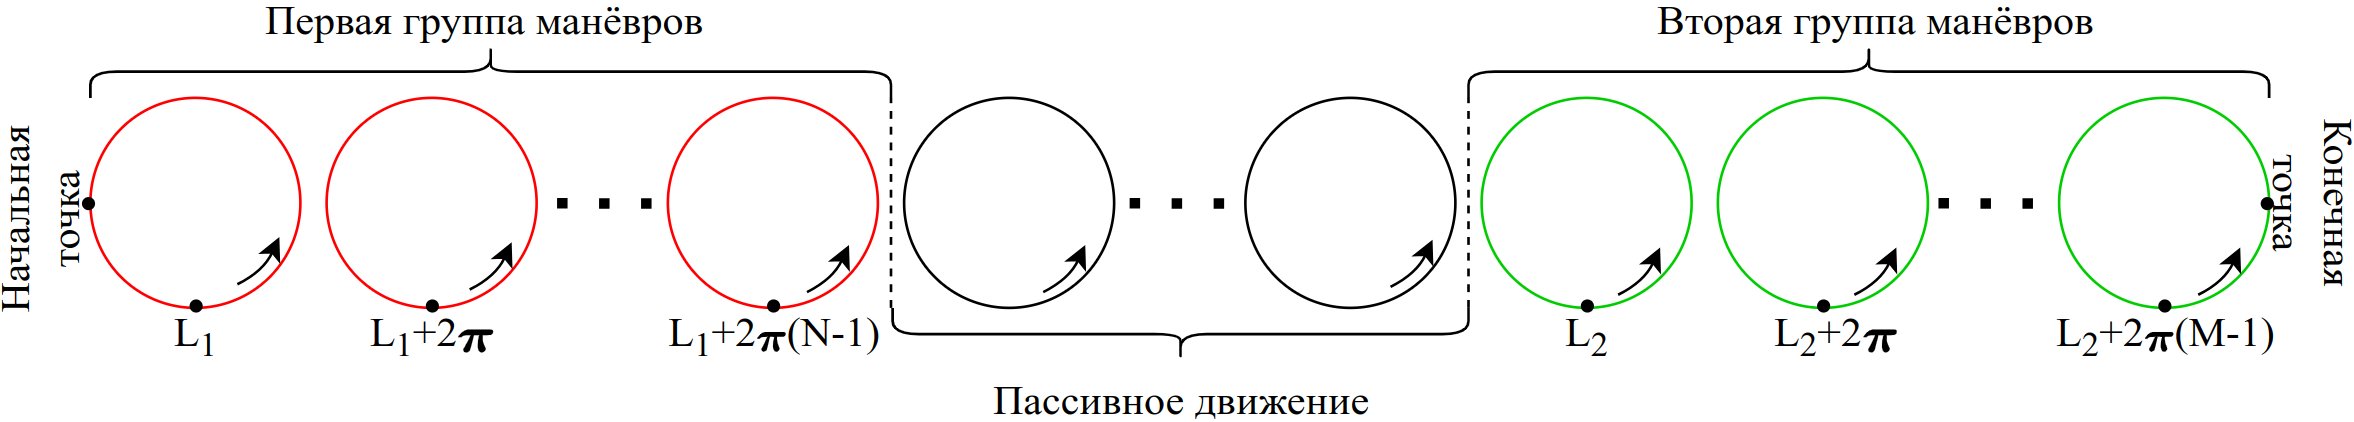
\includegraphics[height=0.24\textheight,keepaspectratio]{images/9/short_rend/plan.png}
\end{center}
\begin{itemize}
    \item Поиск оптимальных точек приложения импульсов для двухимпульсной задачи встречи. Для прогноза движения КА используется численно-аналитический метод, учитывающий сплюснутость Земли. Метод оптимизации - перебор.
    \item На каждой итерации метода перебора для двух фиксированных углов $L_1$ и $L_2$ решается и уточняется задача встречи. Решаемая система имеет следующий вид:
    \begin{equation*}
        \left( \sum_{i=0}^{N-1} M(L_1 + 2 \pi i) \alpha_i \right) \Delta \mathbf{V}_1 + \left( \sum_{i=0}^{K-1} M(L_2 + 2 \pi i) \beta_i \right) \Delta \mathbf{V}_2 = \Delta \mathbf{y}.
    \end{equation*}
\end{itemize}
\end{frame}

\begin{frame}{Пример решения задачи встречи короткой продолжительности}
\begin{center}
    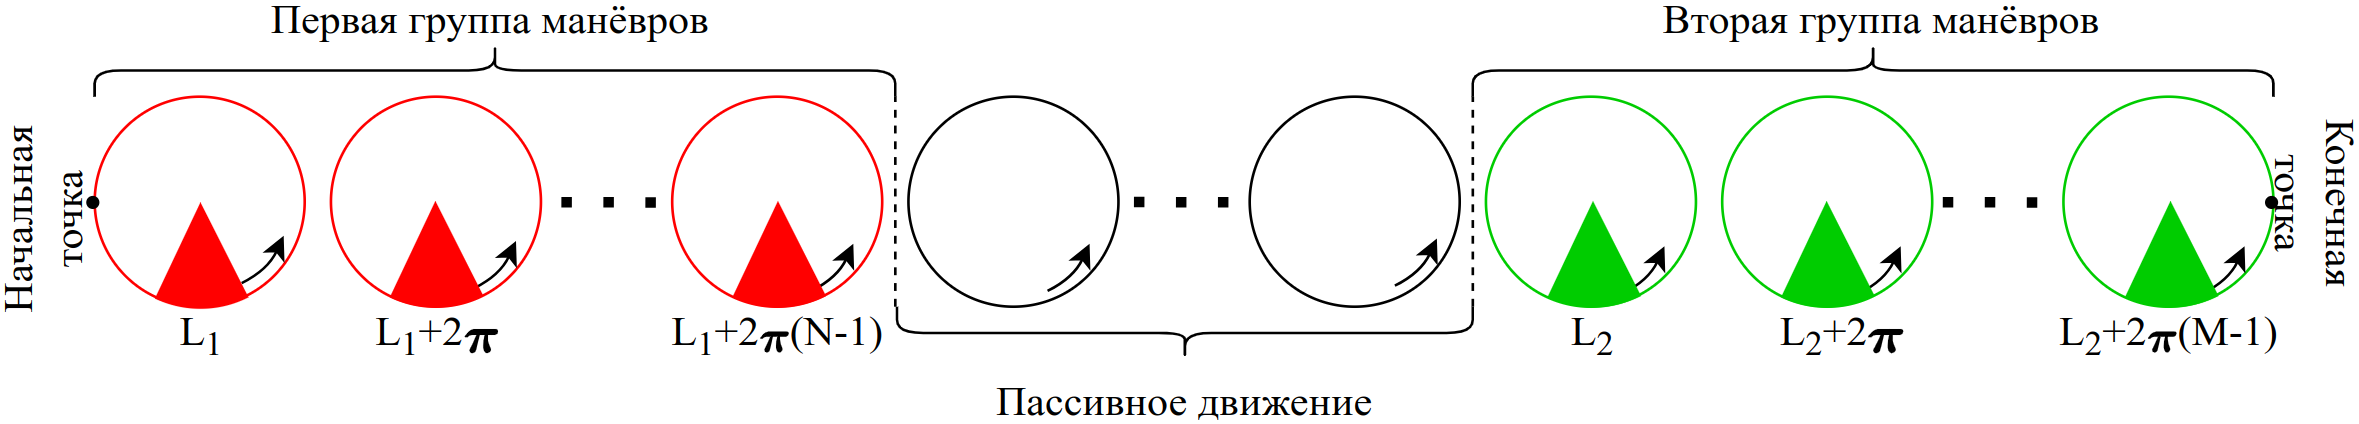
\includegraphics[height=0.24\textheight,keepaspectratio]{images/9/short_rend/plan1.png}
\end{center}
\begin{itemize}
    \item После получения оптимальных точек приложения импульсов $L_1^*$ и $L_2^*$, производится уточнение путём циклического решения системы с учётом необходимого набора возмущающих сил, модели ДУ и использованием численного интегрирования. 
    \item Алгоритм позволяет получить решение, согласно распределению, заданному пользователем. 
\end{itemize}
\end{frame}

\begin{frame}{Пример решения задачи встречи короткой продолжительности}
\begin{columns}[T,totalwidth=\textwidth]
  % Левая колонка
  \begin{column}{0.50\textwidth}
  \begin{center}
      Параметры встречи:
  \end{center}
    \begin{table}[h!]
        \centering
        \begin{tabular}{|c|c|c|}
            \hline
            \textbf{Элементы орбиты} & $\mathbf{y}_{\text{initial}}$ & $\mathbf{y}_{\text{target}}$ \\
            \hline
            $a$, км & 6800 & 6805 \\
            \hline
            $e$ & 0.01 & 0.011 \\
            \hline
            $i$, $^\circ$ & 90 & 90 \\
            \hline
            $\omega$, $^\circ$ & 30 & 30.1 \\
            \hline
            $\Omega$, $^\circ$ & 30 & 30.1 \\
            \hline
            $\nu$, $^\circ$ & 0 & 355 \\
            \hline
            \multicolumn{3}{|c|}{$\Delta t = 2$ дня} \\
            \hline
            \multicolumn{3}{|c|}{\textbf{Модель сил}} \\
            \hline
            \multicolumn{3}{|c|}{Гравитационный потенциал (16 × 16),} \\
            \multicolumn{3}{|c|}{сопротивление атмосферы,} \\
            \multicolumn{3}{|c|}{притяжение третьих тел,} \\
            \multicolumn{3}{|c|}{давление радиационного излучения} \\
            \hline
            \multicolumn{3}{|c|}{\textbf{Ограничения}} \\
            \hline
            Ускорение $a$, м/с$^2$ & \multicolumn{2}{c|}{0.005} \\
            \hline
            Макс. длит. имп. $t_{\max}$, c & \multicolumn{2}{c|}{500} \\
            \hline
            $S/m$, м$^2$/кг & \multicolumn{2}{c|}{0.01} \\
            \hline
        \end{tabular}
    \end{table}
  \end{column}

  % Правая колонка
  \begin{column}{0.50\textwidth}
    \begin{center}
        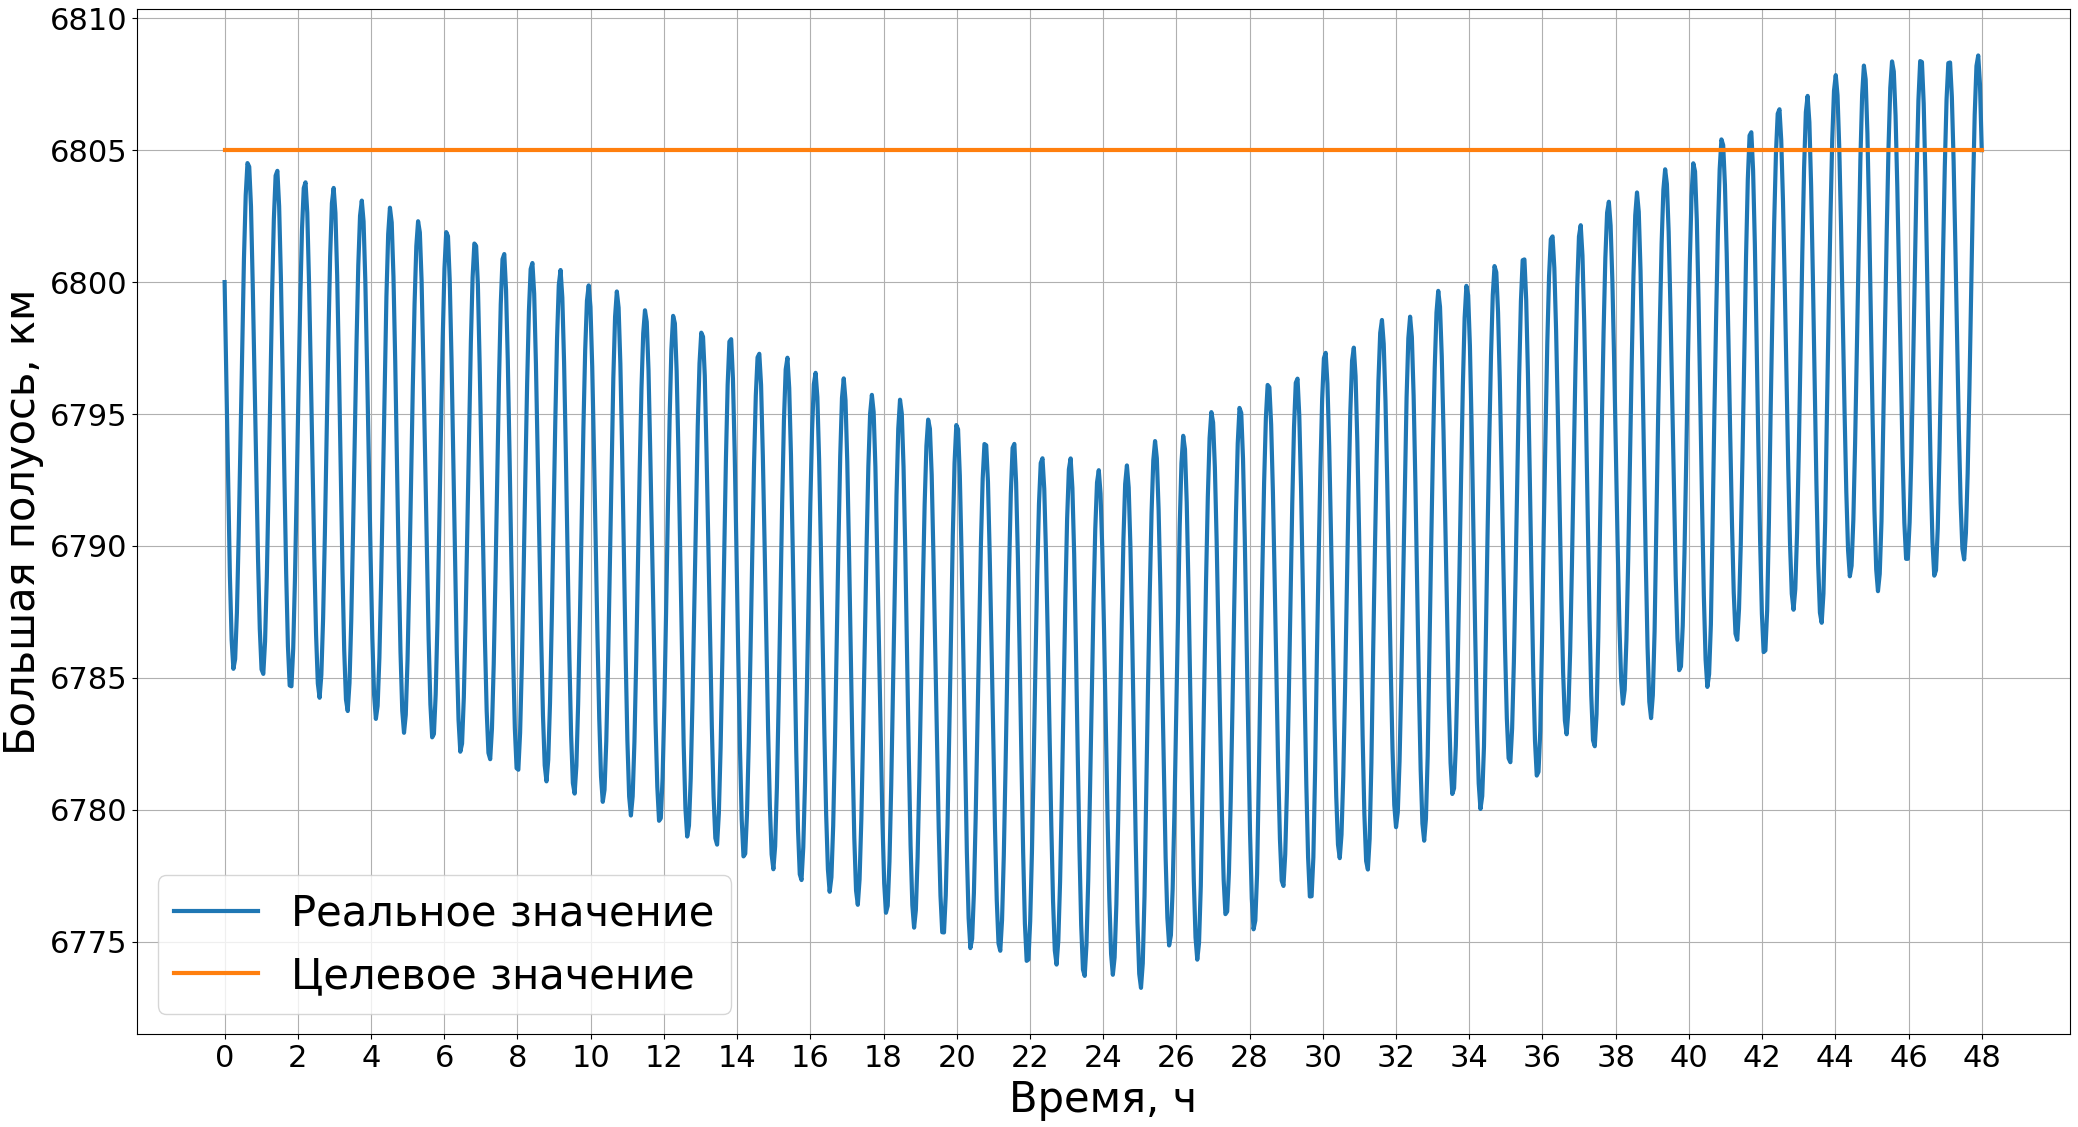
\includegraphics[height=0.37\textheight,keepaspectratio]{images/9/short_rend/a.png}
        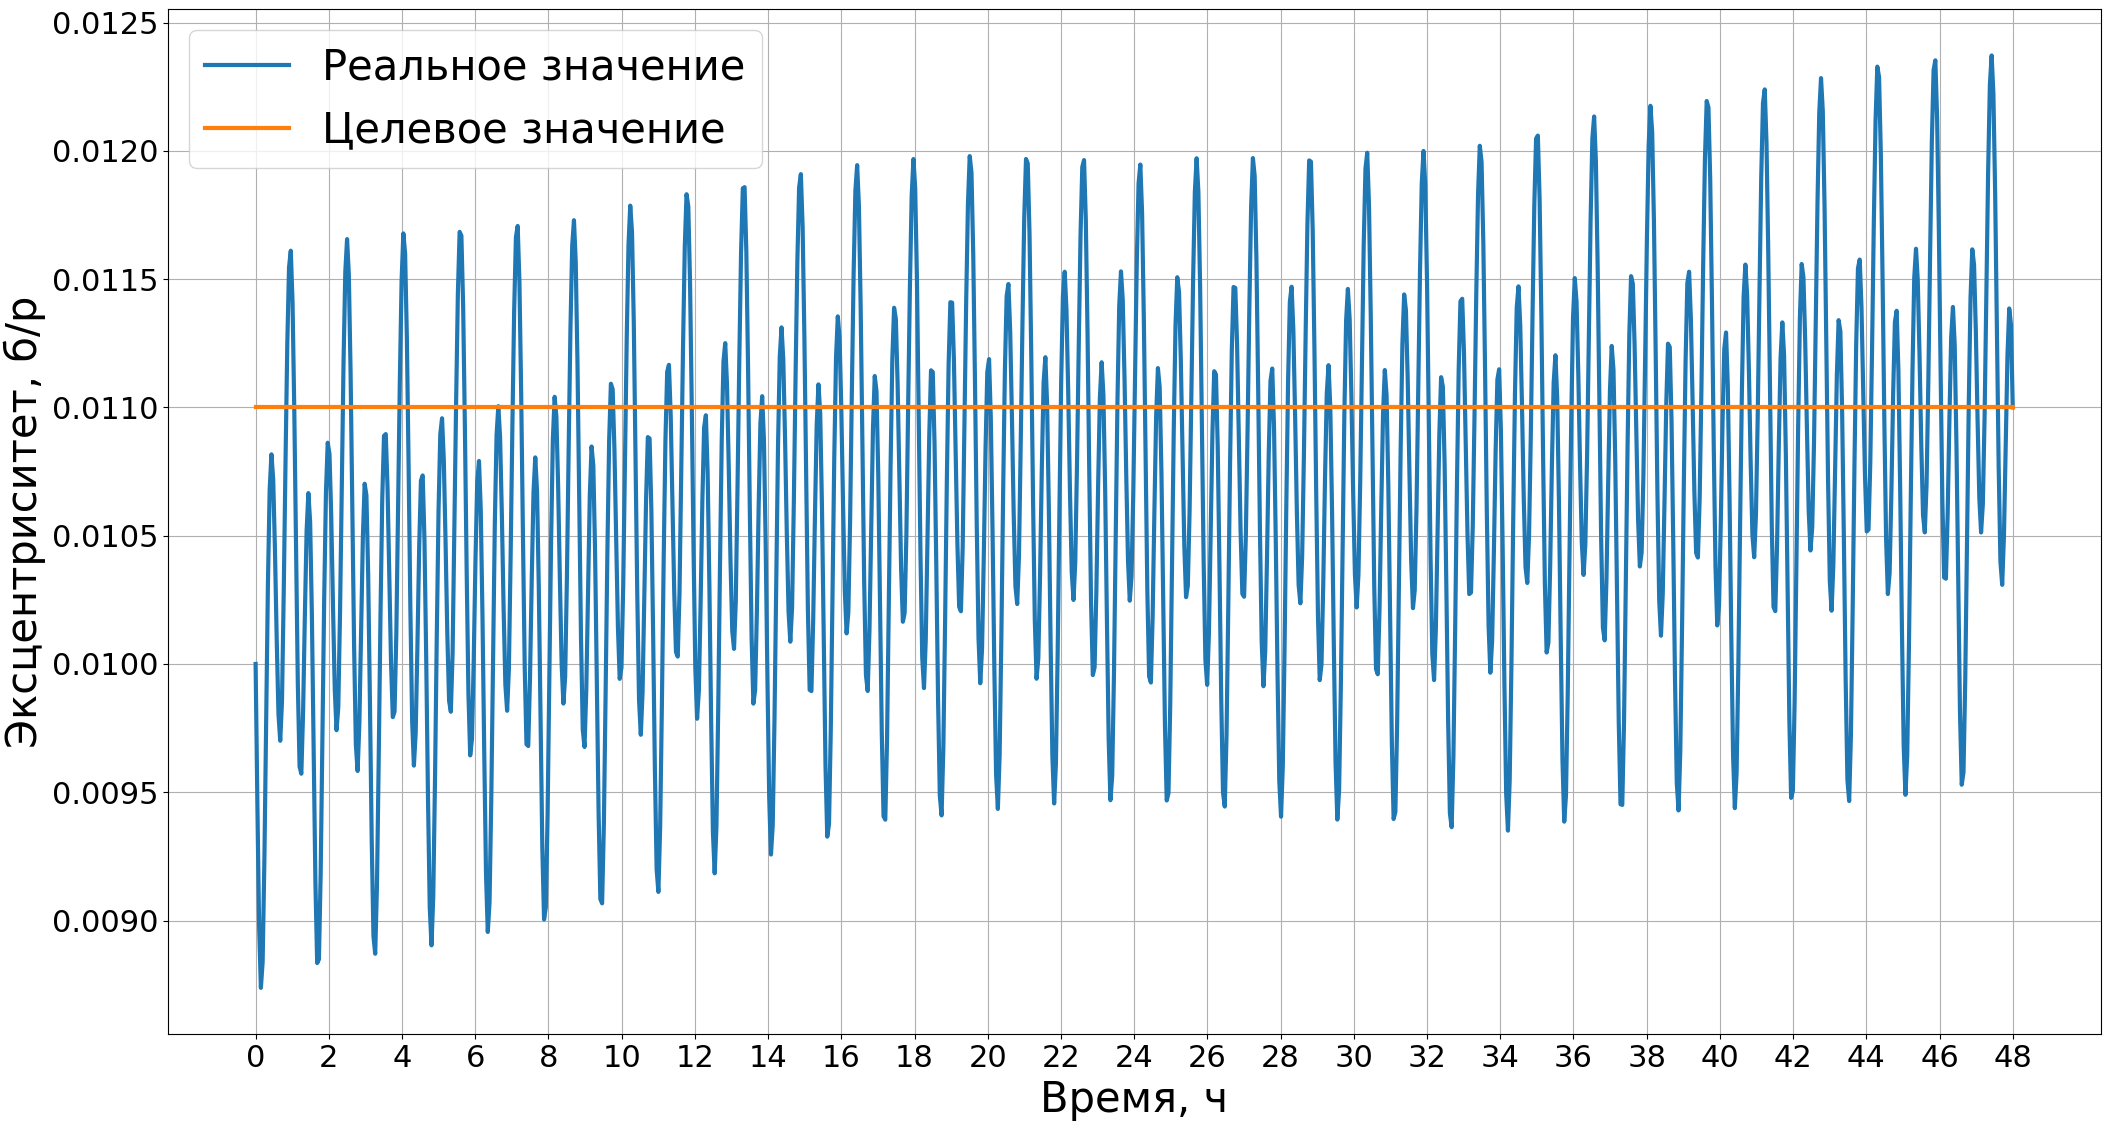
\includegraphics[height=0.37\textheight,keepaspectratio]{images/9/short_rend/e.png}
    \end{center}
  \end{column}
\end{columns}
\end{frame}

\begin{frame}{Пример решения задачи встречи короткой продолжительности}
\begin{columns}[T,totalwidth=\textwidth]
  % Левая колонка
  \begin{column}{0.50\textwidth}
    \begin{center}
        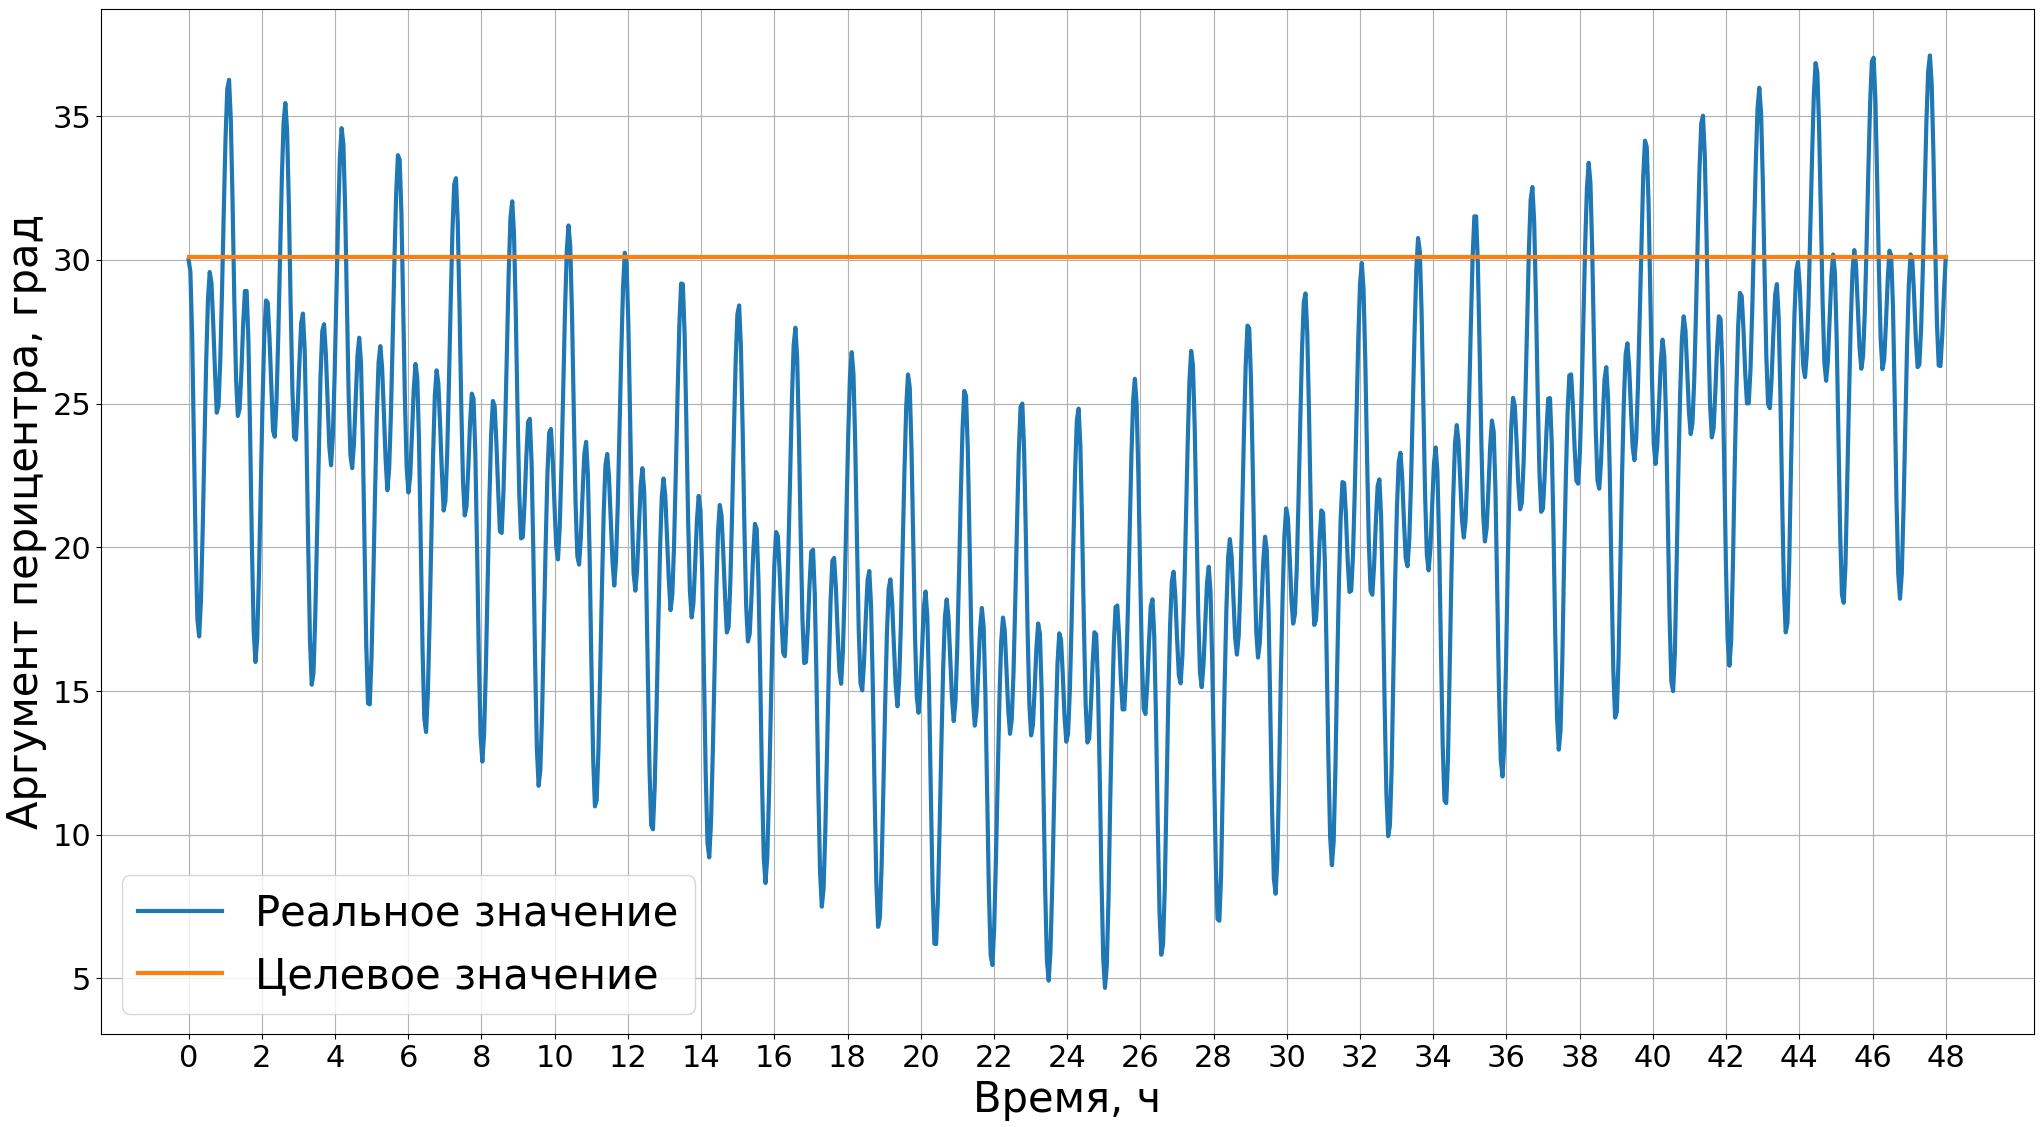
\includegraphics[height=0.37\textheight,keepaspectratio]{images/9/short_rend/w.png}
        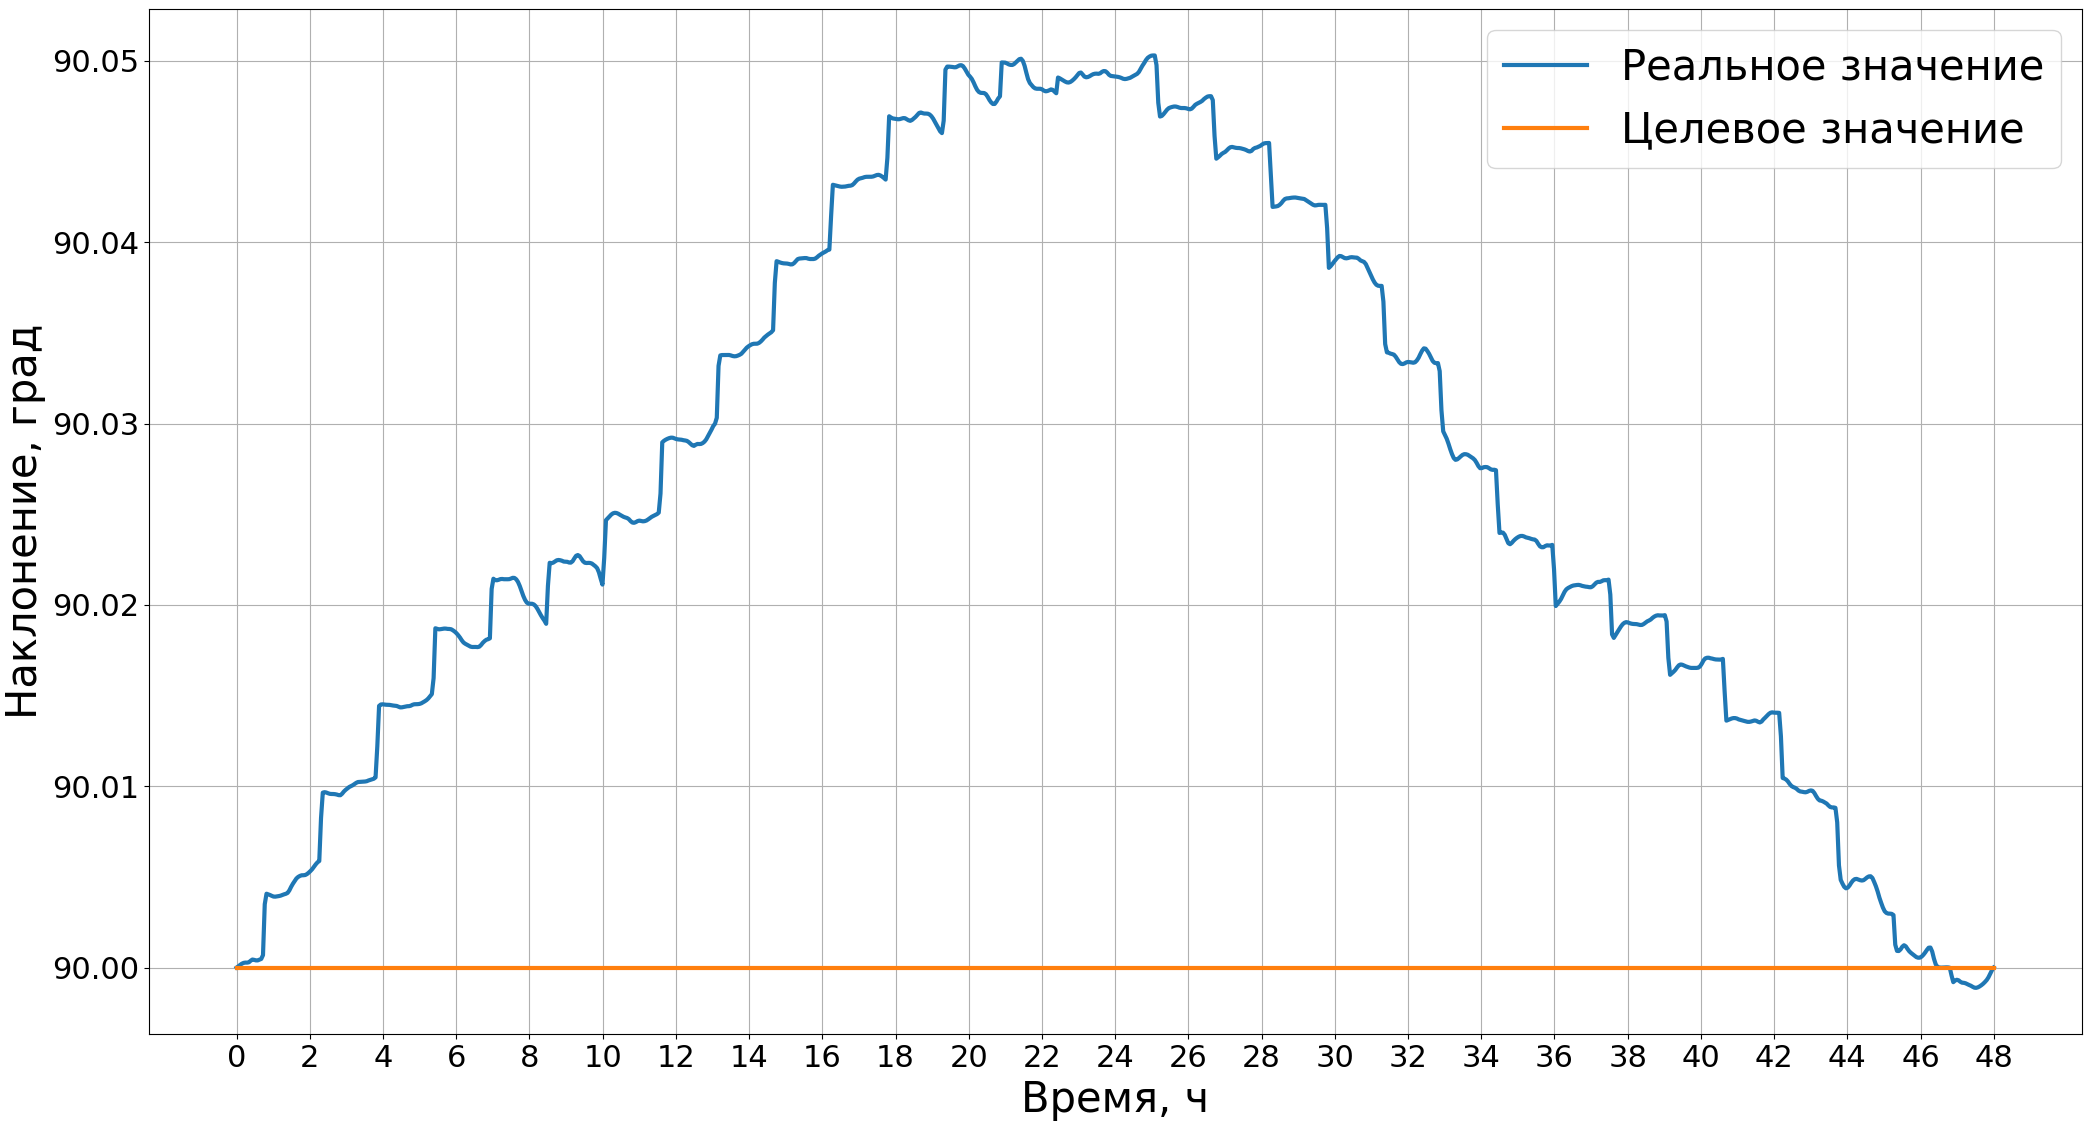
\includegraphics[height=0.37\textheight,keepaspectratio]{images/9/short_rend/i.png}
    \end{center}
  \end{column}

  % Правая колонка
  \begin{column}{0.50\textwidth}
    \begin{center}
        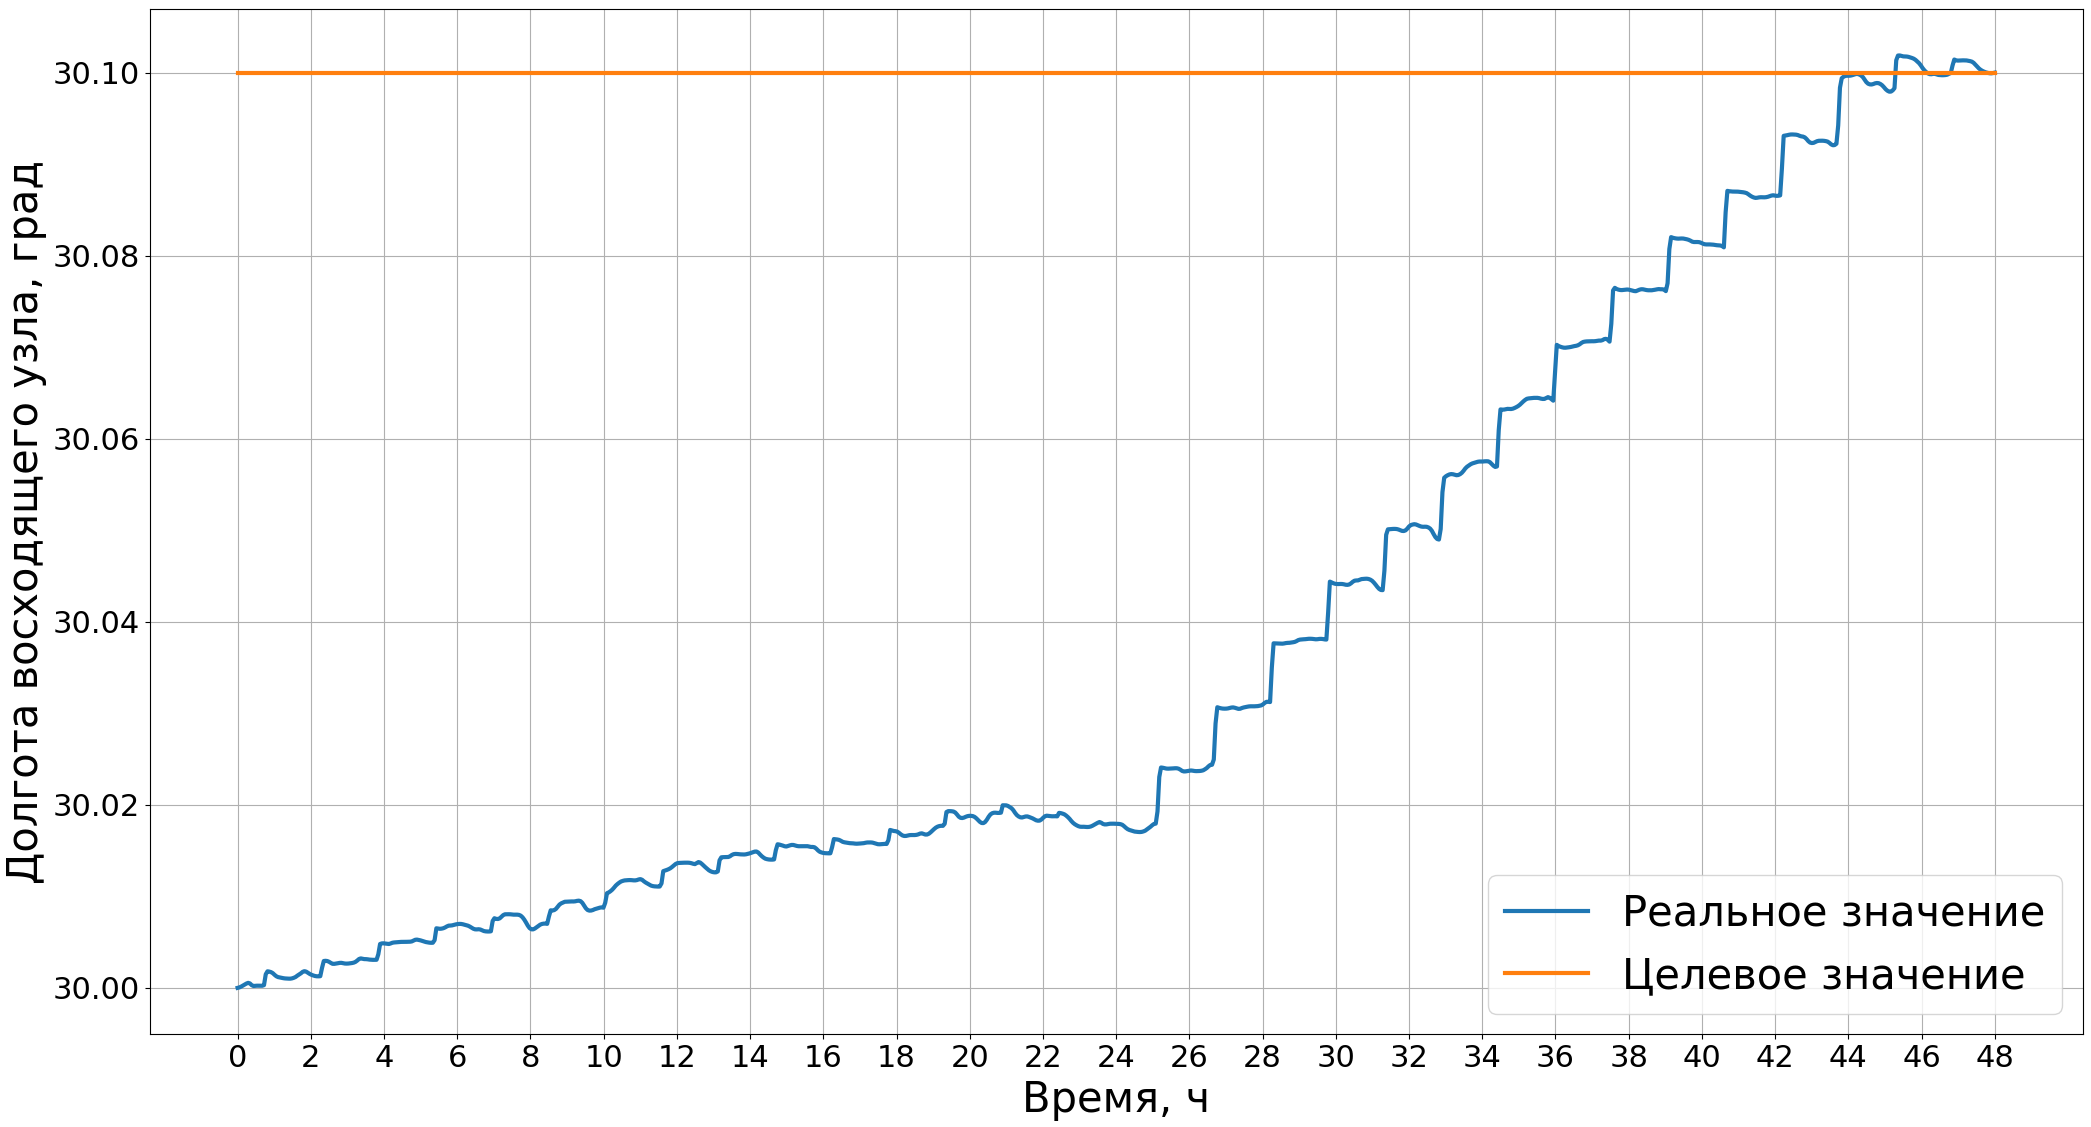
\includegraphics[height=0.37\textheight,keepaspectratio]{images/9/short_rend/raan.png}
        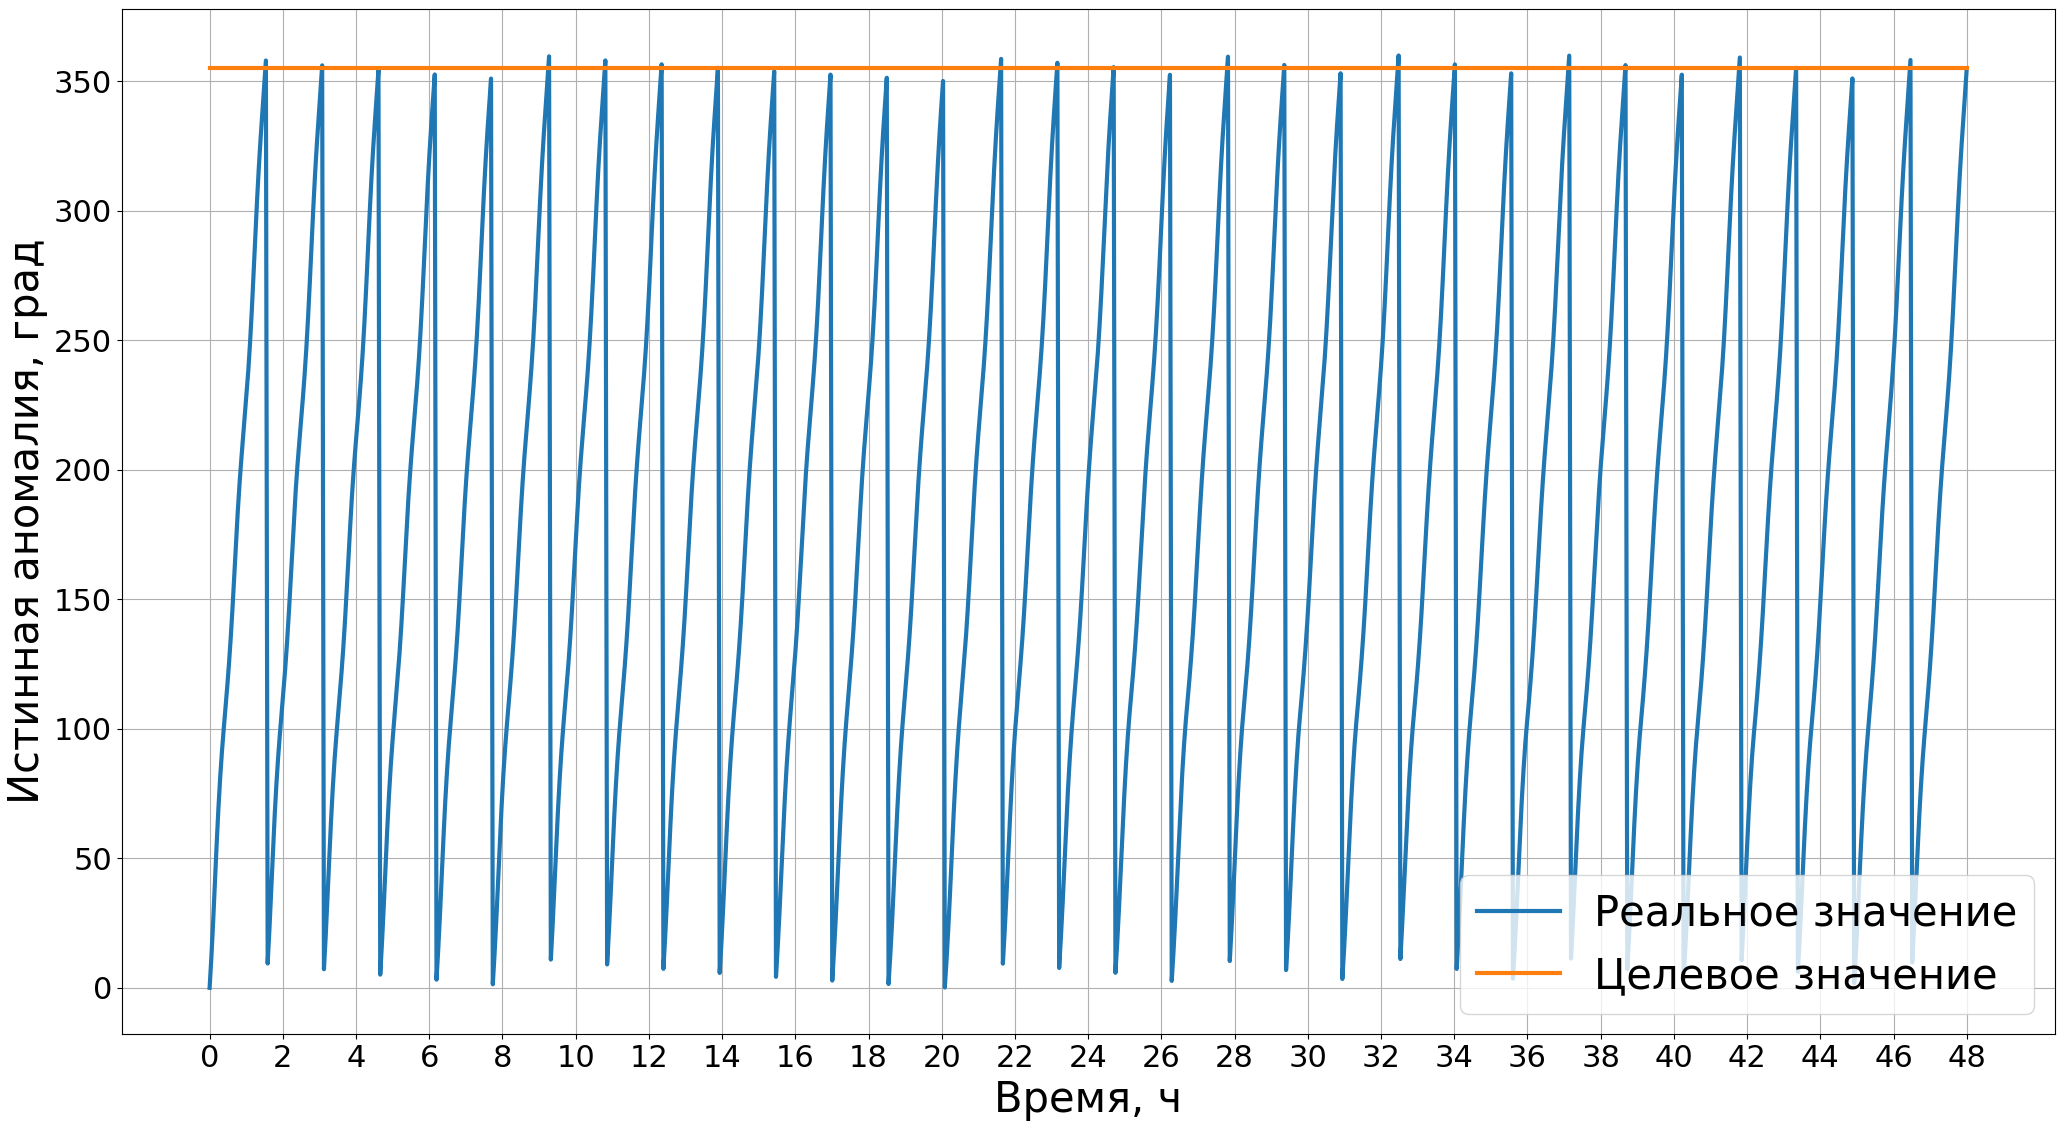
\includegraphics[height=0.37\textheight,keepaspectratio]{images/9/short_rend/nu.png}
    \end{center}
  \end{column}
\end{columns}
\end{frame}

\begin{frame}{Пример решения задачи встречи короткой продолжительности}
\begin{center}
    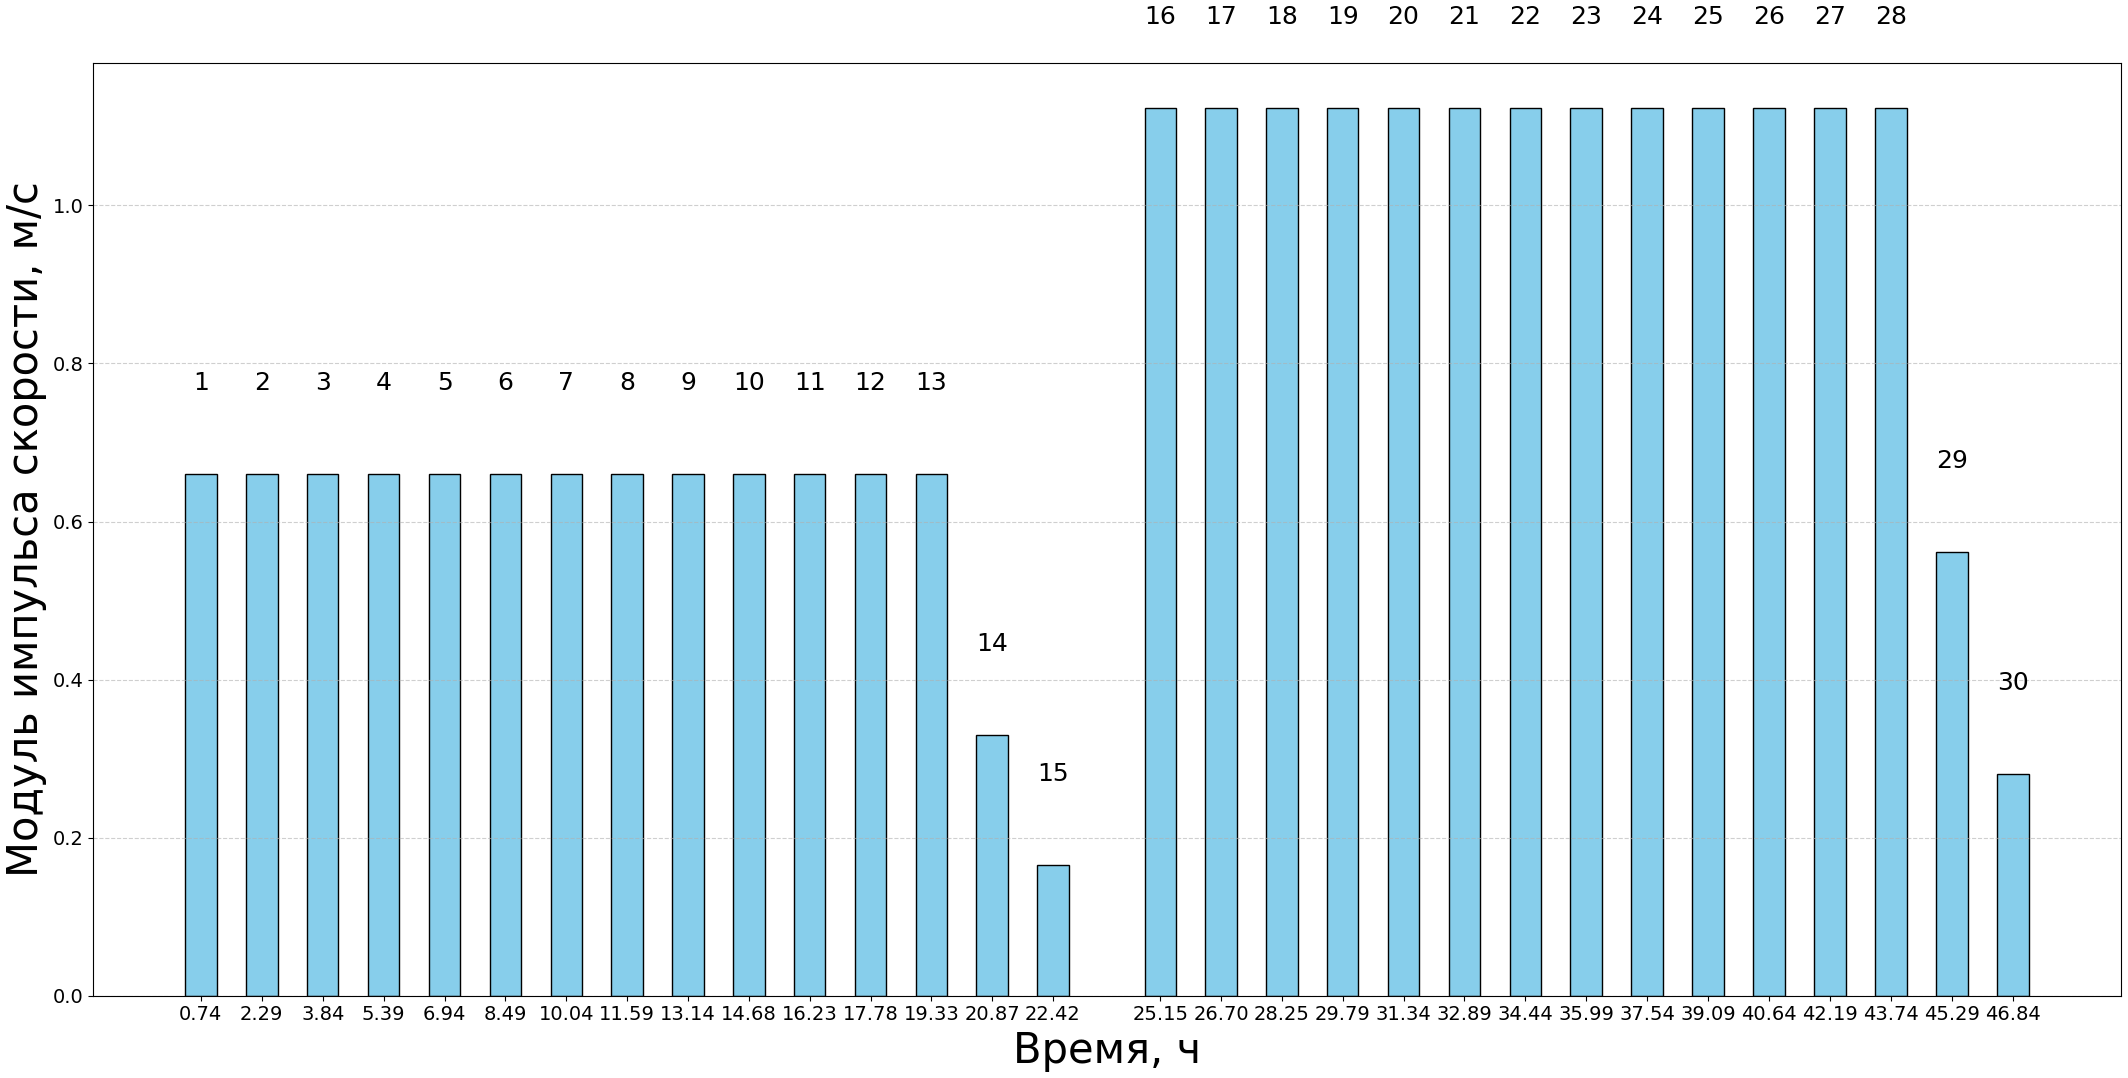
\includegraphics[height=0.65\textheight,keepaspectratio]{images/9/short_rend/v_distribution.png}
\end{center}
\end{frame}

\begin{frame}{Пример решения задачи встречи большой продолжительности}
\begin{center}
    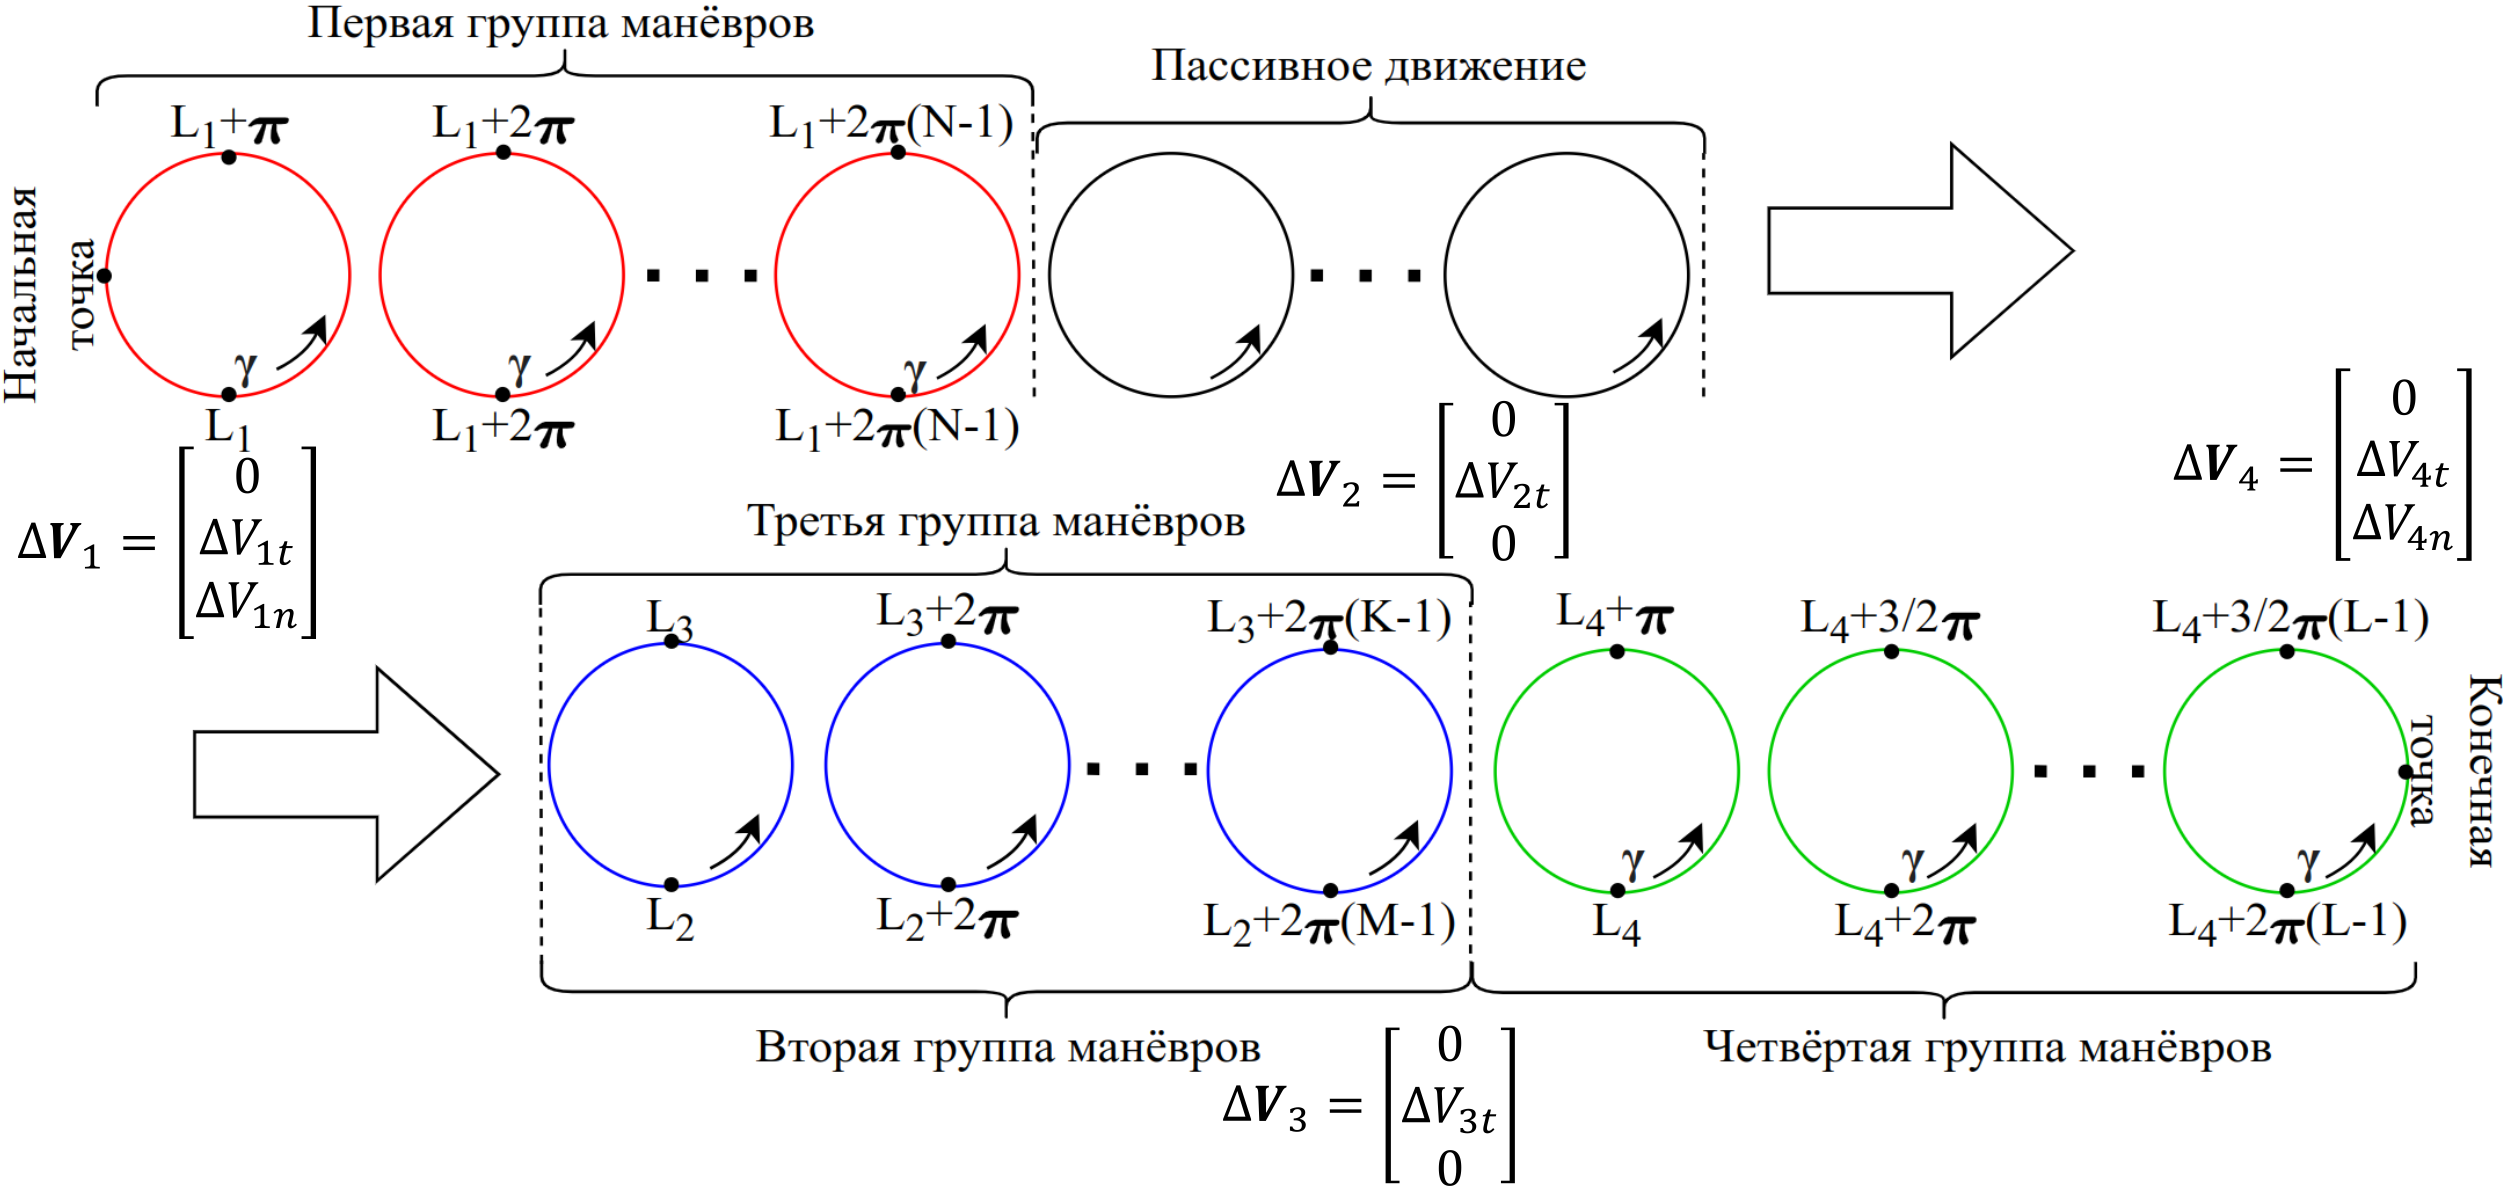
\includegraphics[height=0.50\textheight,keepaspectratio]{images/9/long_rend/plan.png}
\end{center}
\begin{itemize}
    \item Поиск оптимальных точек приложения второй и третьей групп импульсов. Метод оптимизации - перебор. \\
    \item На каждой итерации метода перебора для двух фиксированных углов $L_2$ и $L_3$ решается и уточняется задача встречи. Решаемая система имеет следующий вид:
    \begin{align*}
        &\left( \sum_{i=0}^{N-1} M^{tn}(L_{1i}) \alpha_i \right) \Delta \mathbf{V}_1 + \left( \sum_{i=0}^{K-1} M^{t}(L_{2i}) \beta_i \right) \Delta \mathbf{V}_2 + \\
        &+ \left( \sum_{i=0}^{P-1} M^{t}(L_{3i}) \gamma_i \right) \Delta \mathbf{V}_3 + \left( \sum_{i=0}^{Q-1} M^{tn}(L_{2i}) \delta_i \right) \Delta \mathbf{V}_4 = \Delta \mathbf{y}.
    \end{align*}
\end{itemize}
\end{frame}

\begin{frame}{Пример решения задачи встречи большой продолжительности}
\begin{center}
    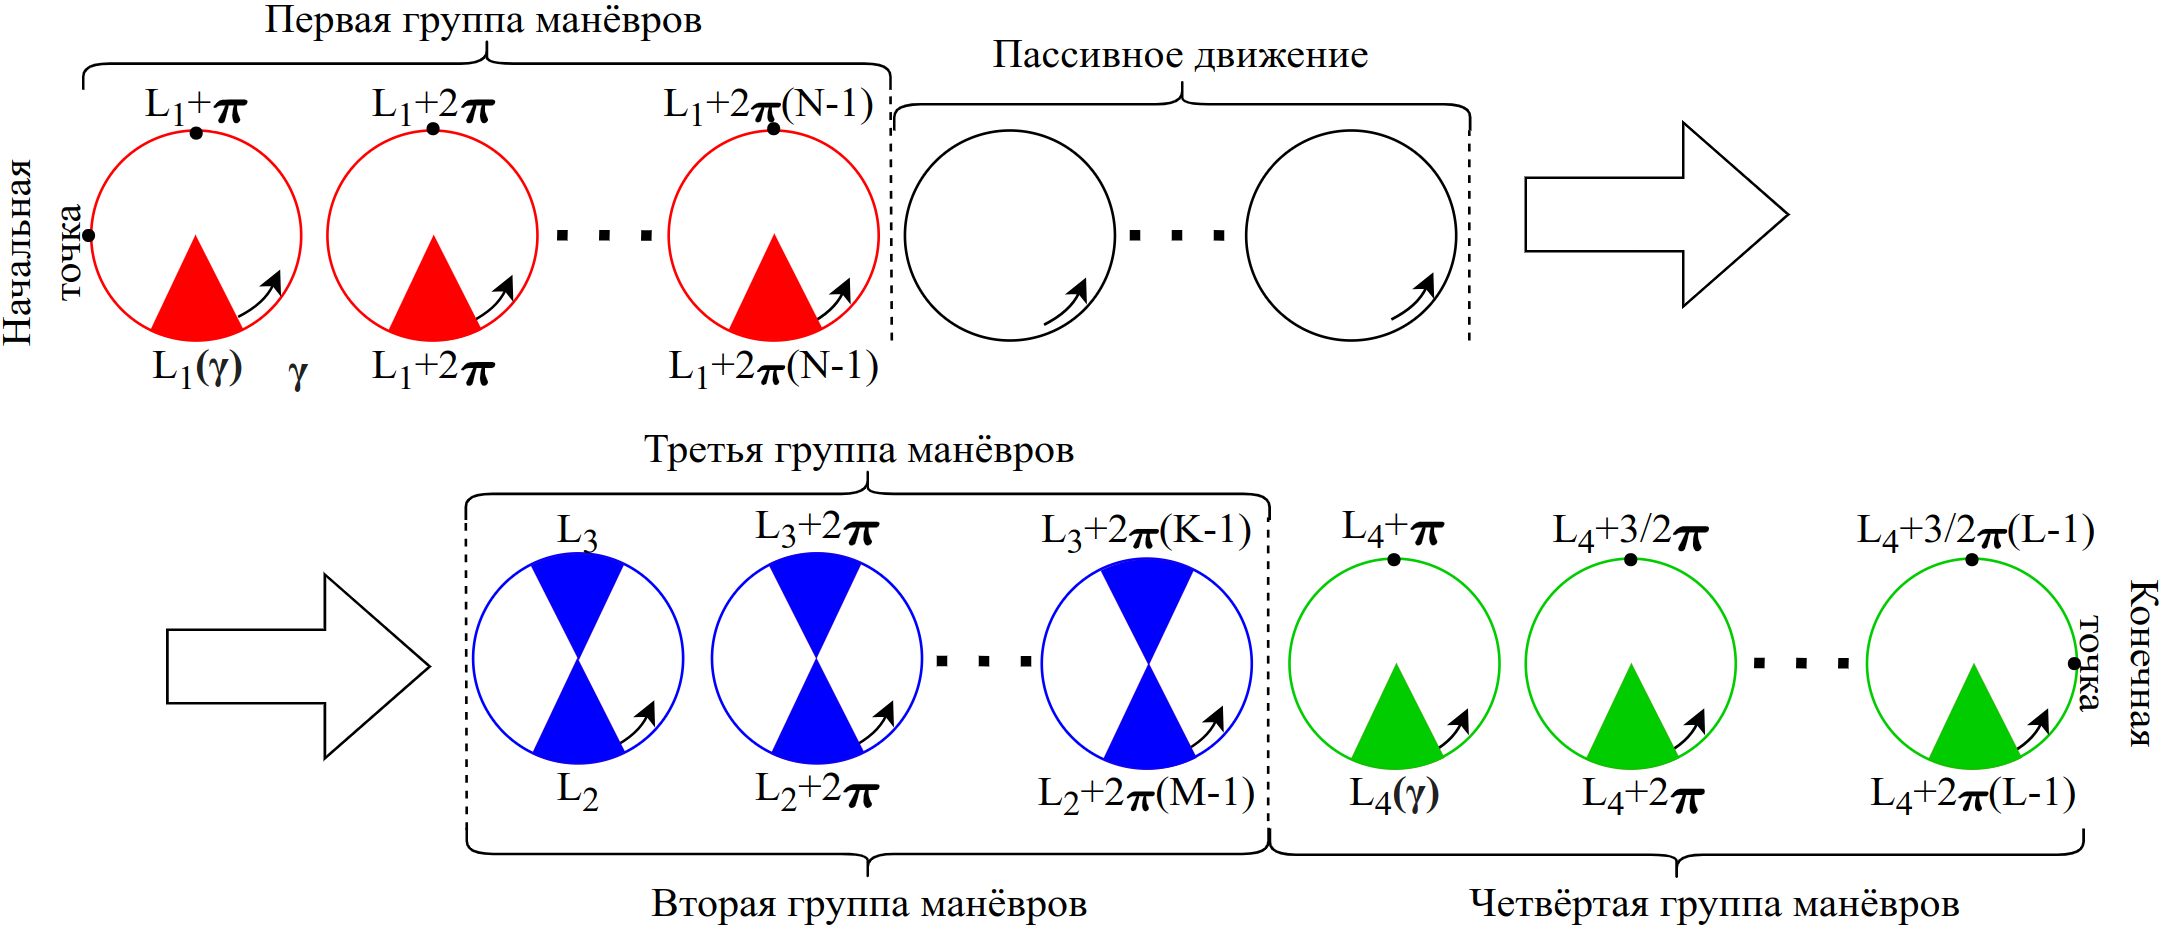
\includegraphics[height=0.55\textheight,keepaspectratio]{images/9/long_rend/plan1.png}
\end{center}
\begin{itemize}
    \item После получения оптимальных точек приложения импульсов $L_2^*$ и $L_3^*$, производится уточнение путём циклического решения системы с учётом необходимого набора возмущающих сил, модели ДУ и использованием численного интегрирования. 
    \item Алгоритм позволяет получить решение, согласно распределению, заданному пользователем. 
\end{itemize}
\end{frame}

\begin{frame}{Пример решения задачи встречи большой продолжительности}
\begin{columns}[T,totalwidth=\textwidth]
  % Левая колонка
  \begin{column}{0.50\textwidth}
  \begin{center}
      Параметры встречи:
  \end{center}
    \begin{table}[h!]
        \centering
        \begin{tabular}{|c|c|c|}
            \hline
            \textbf{Элементы орбиты} & $\mathbf{y}_{\text{initial}}$ & $\Delta \mathbf{y}$ \\
            \hline
            $a$, км & 6800 & 1 \\
            \hline
            $e$ & 0.01 & 0.001 \\
            \hline
            $i$, $^\circ$ & 80 & 0.01 \\
            \hline
            $\omega$, $^\circ$ & 300 & 1 \\
            \hline
            $\Omega$, $^\circ$ & 300 & 1 \\
            \hline
            $\nu$, $^\circ$ & 30 & 10 \\
            \hline
            \multicolumn{3}{|c|}{$\Delta t = 50$ дня} \\
            \hline
            \multicolumn{3}{|c|}{\textbf{Модель сил}} \\
            \hline
            \multicolumn{3}{|c|}{Гравитационный потенциал (16 × 16),} \\
            \multicolumn{3}{|c|}{сопротивление атмосферы,} \\
            \multicolumn{3}{|c|}{притяжение третьих тел,} \\
            \multicolumn{3}{|c|}{давление радиационного излучения} \\
            \hline
            \multicolumn{3}{|c|}{\textbf{Ограничения}} \\
            \hline
            Ускорение $a$, м/с$^2$ & \multicolumn{2}{c|}{0.05} \\
            \hline
            Макс. длит. имп. $t_{\max}$, c & \multicolumn{2}{c|}{1000} \\
            \hline
            $S/m$, м$^2$/кг & \multicolumn{2}{c|}{0.01} \\
            \hline
        \end{tabular}
    \end{table}
  \end{column}

  % Правая колонка
  \begin{column}{0.50\textwidth}
    \begin{center}
        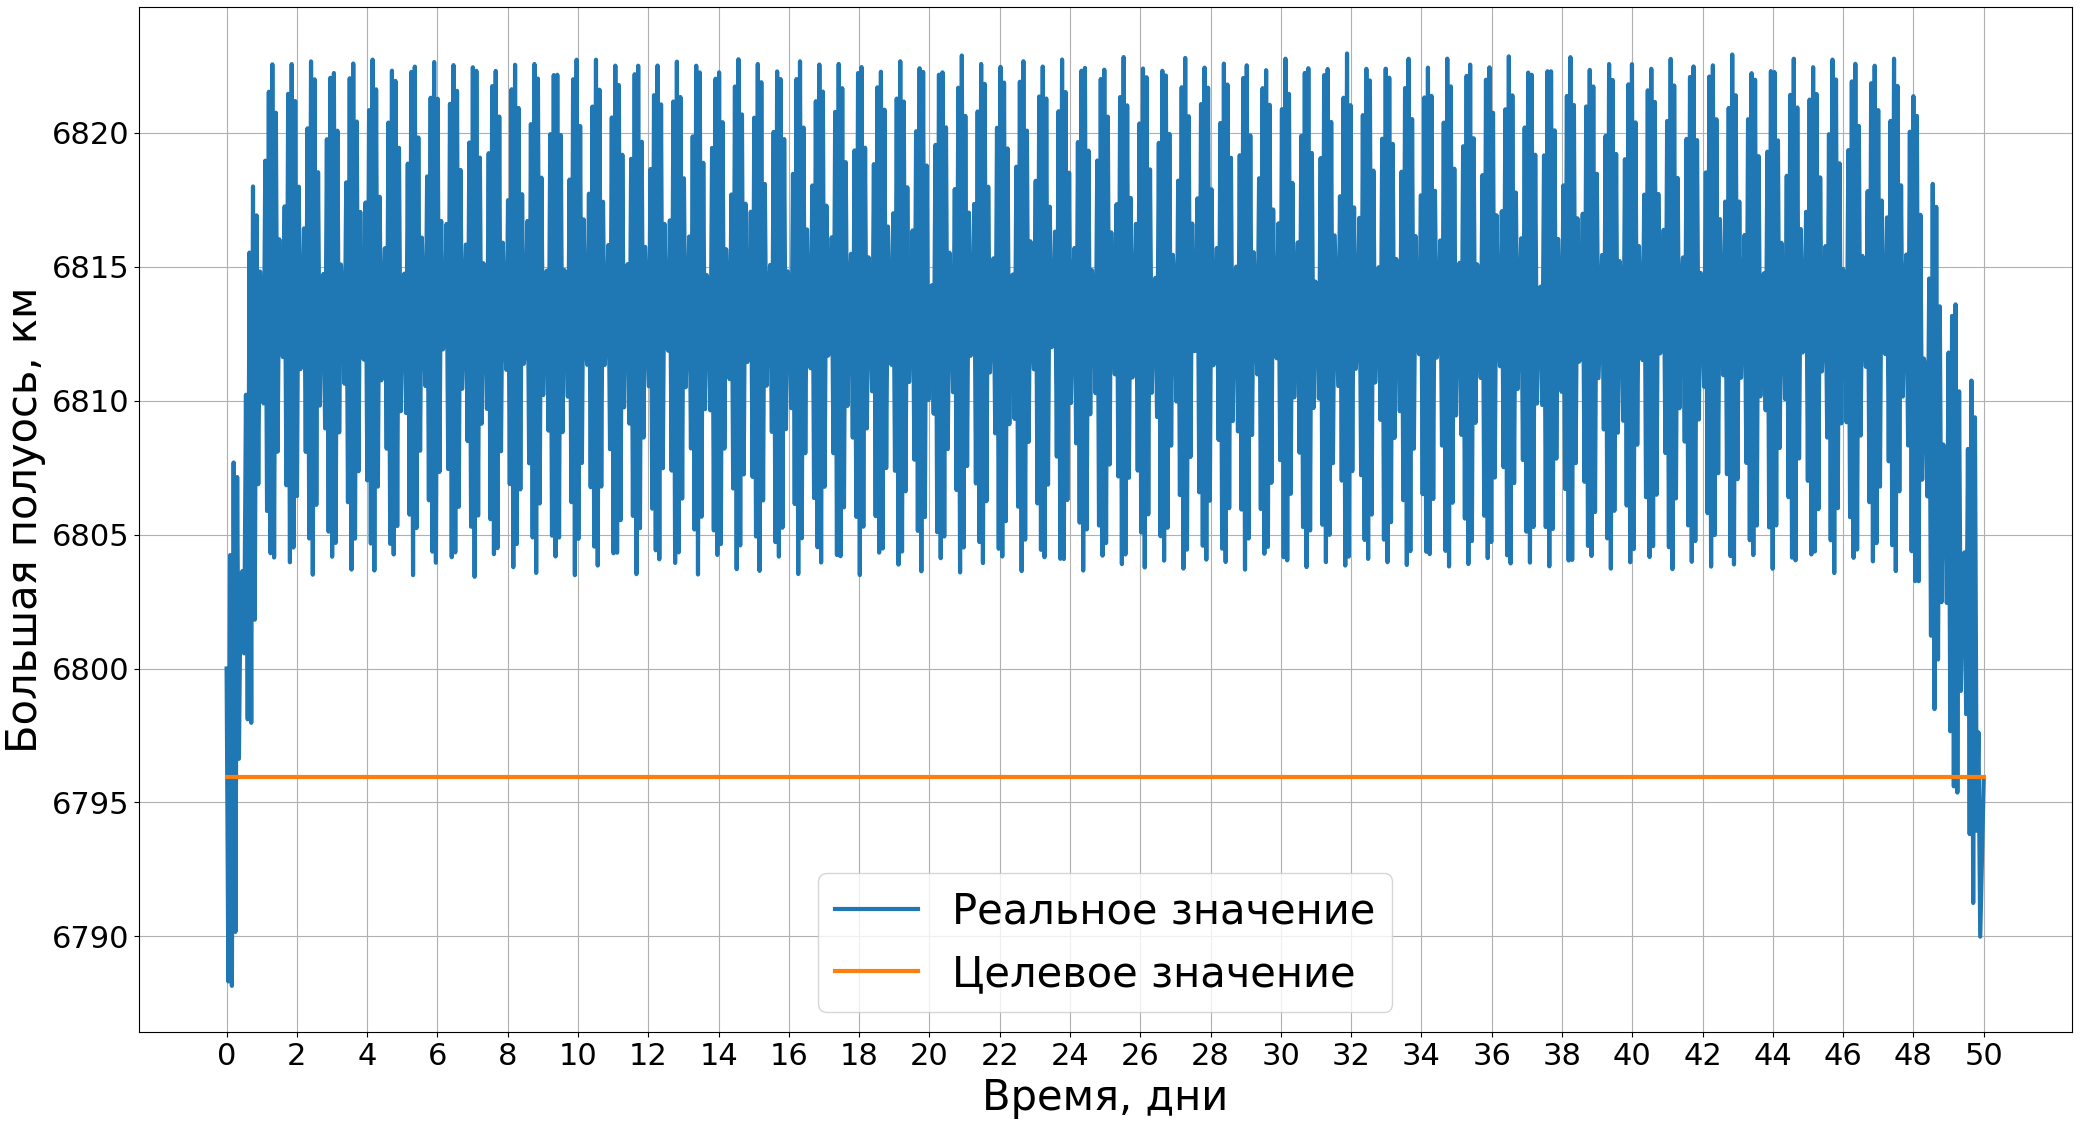
\includegraphics[height=0.37\textheight,keepaspectratio]{images/9/long_rend/a.png}
        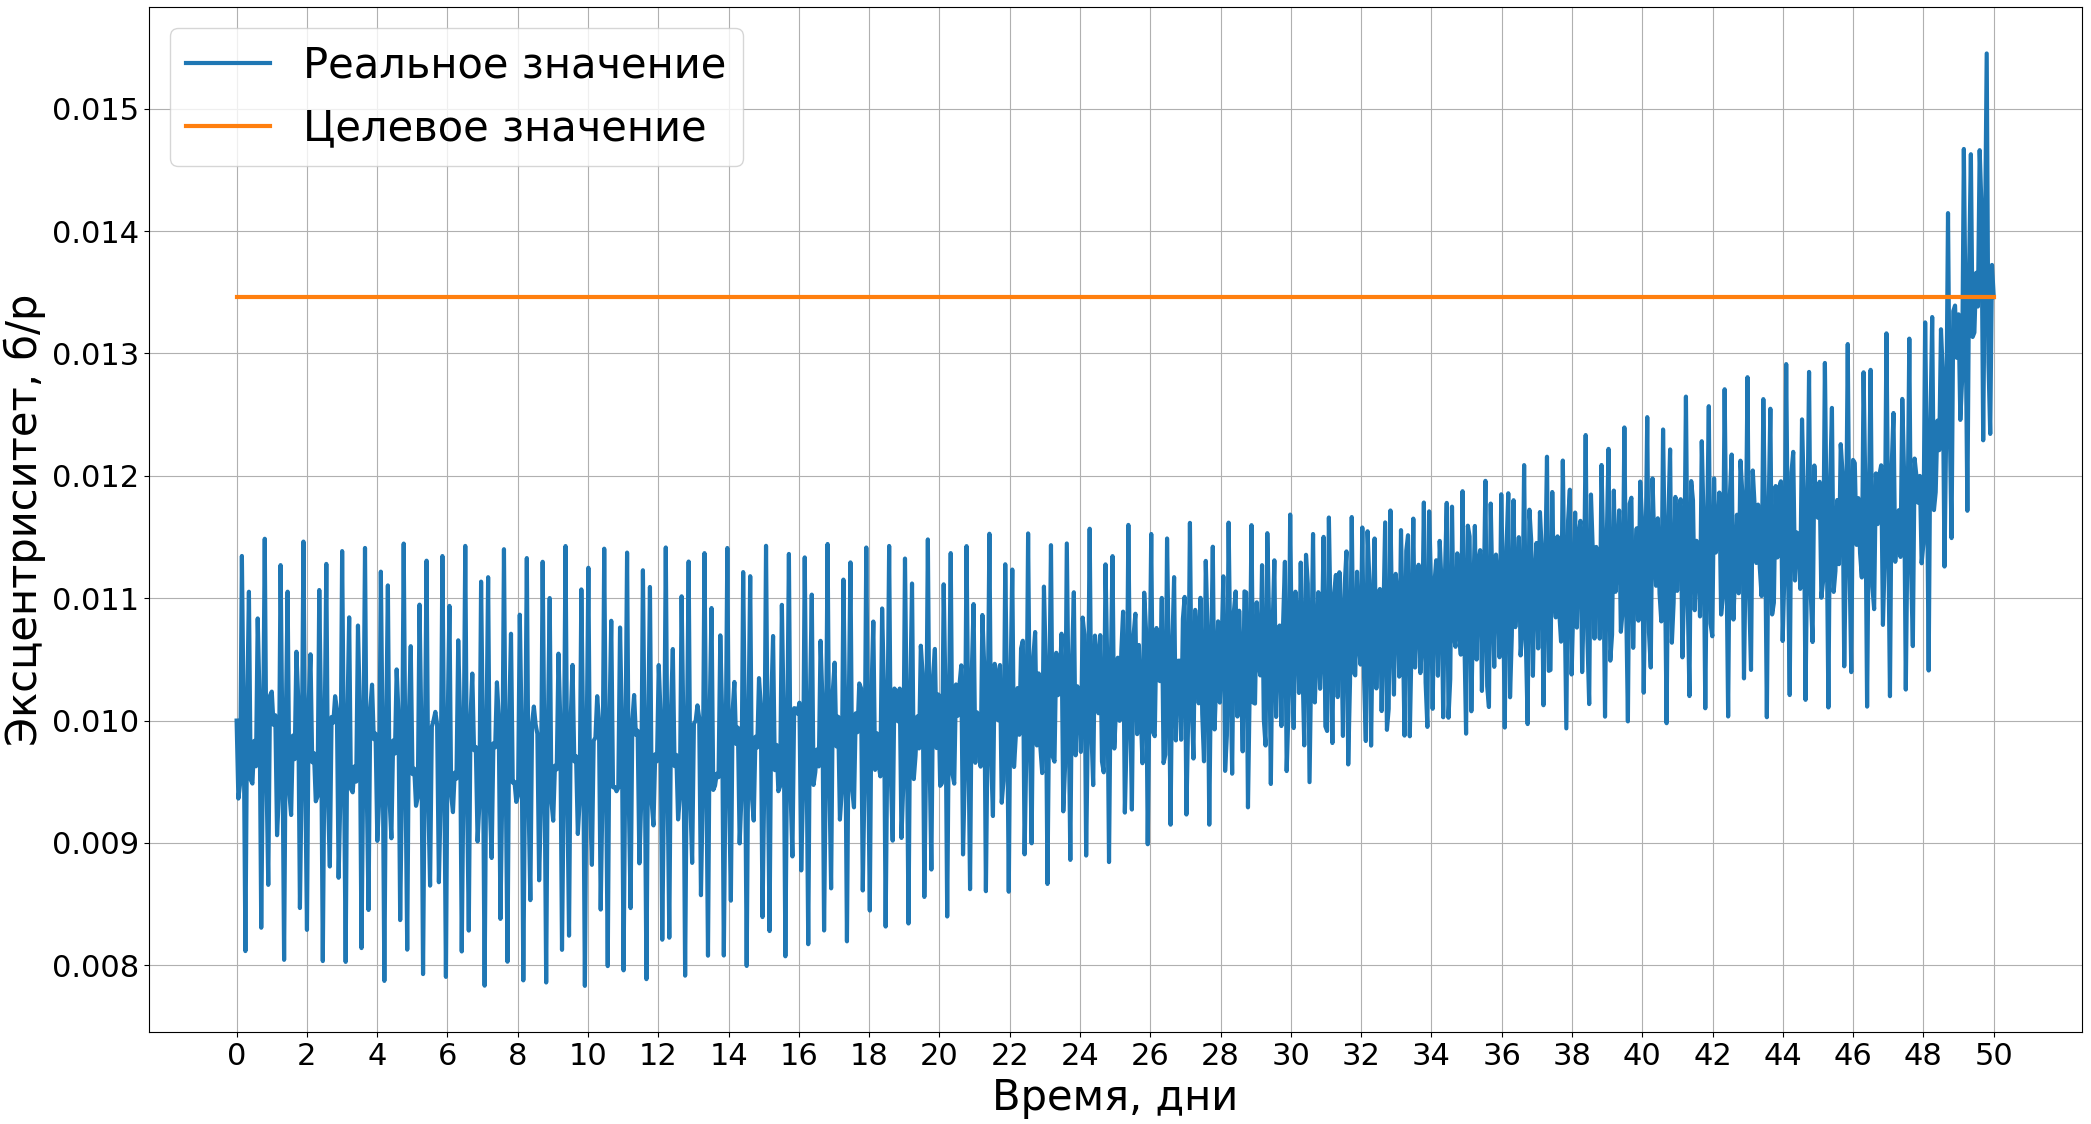
\includegraphics[height=0.37\textheight,keepaspectratio]{images/9/long_rend/e.png}
    \end{center}
  \end{column}
\end{columns}
\end{frame}

\begin{frame}{Пример решения задачи встречи большой продолжительности}
\begin{columns}[T,totalwidth=\textwidth]
  % Левая колонка
  \begin{column}{0.50\textwidth}
    \begin{center}
        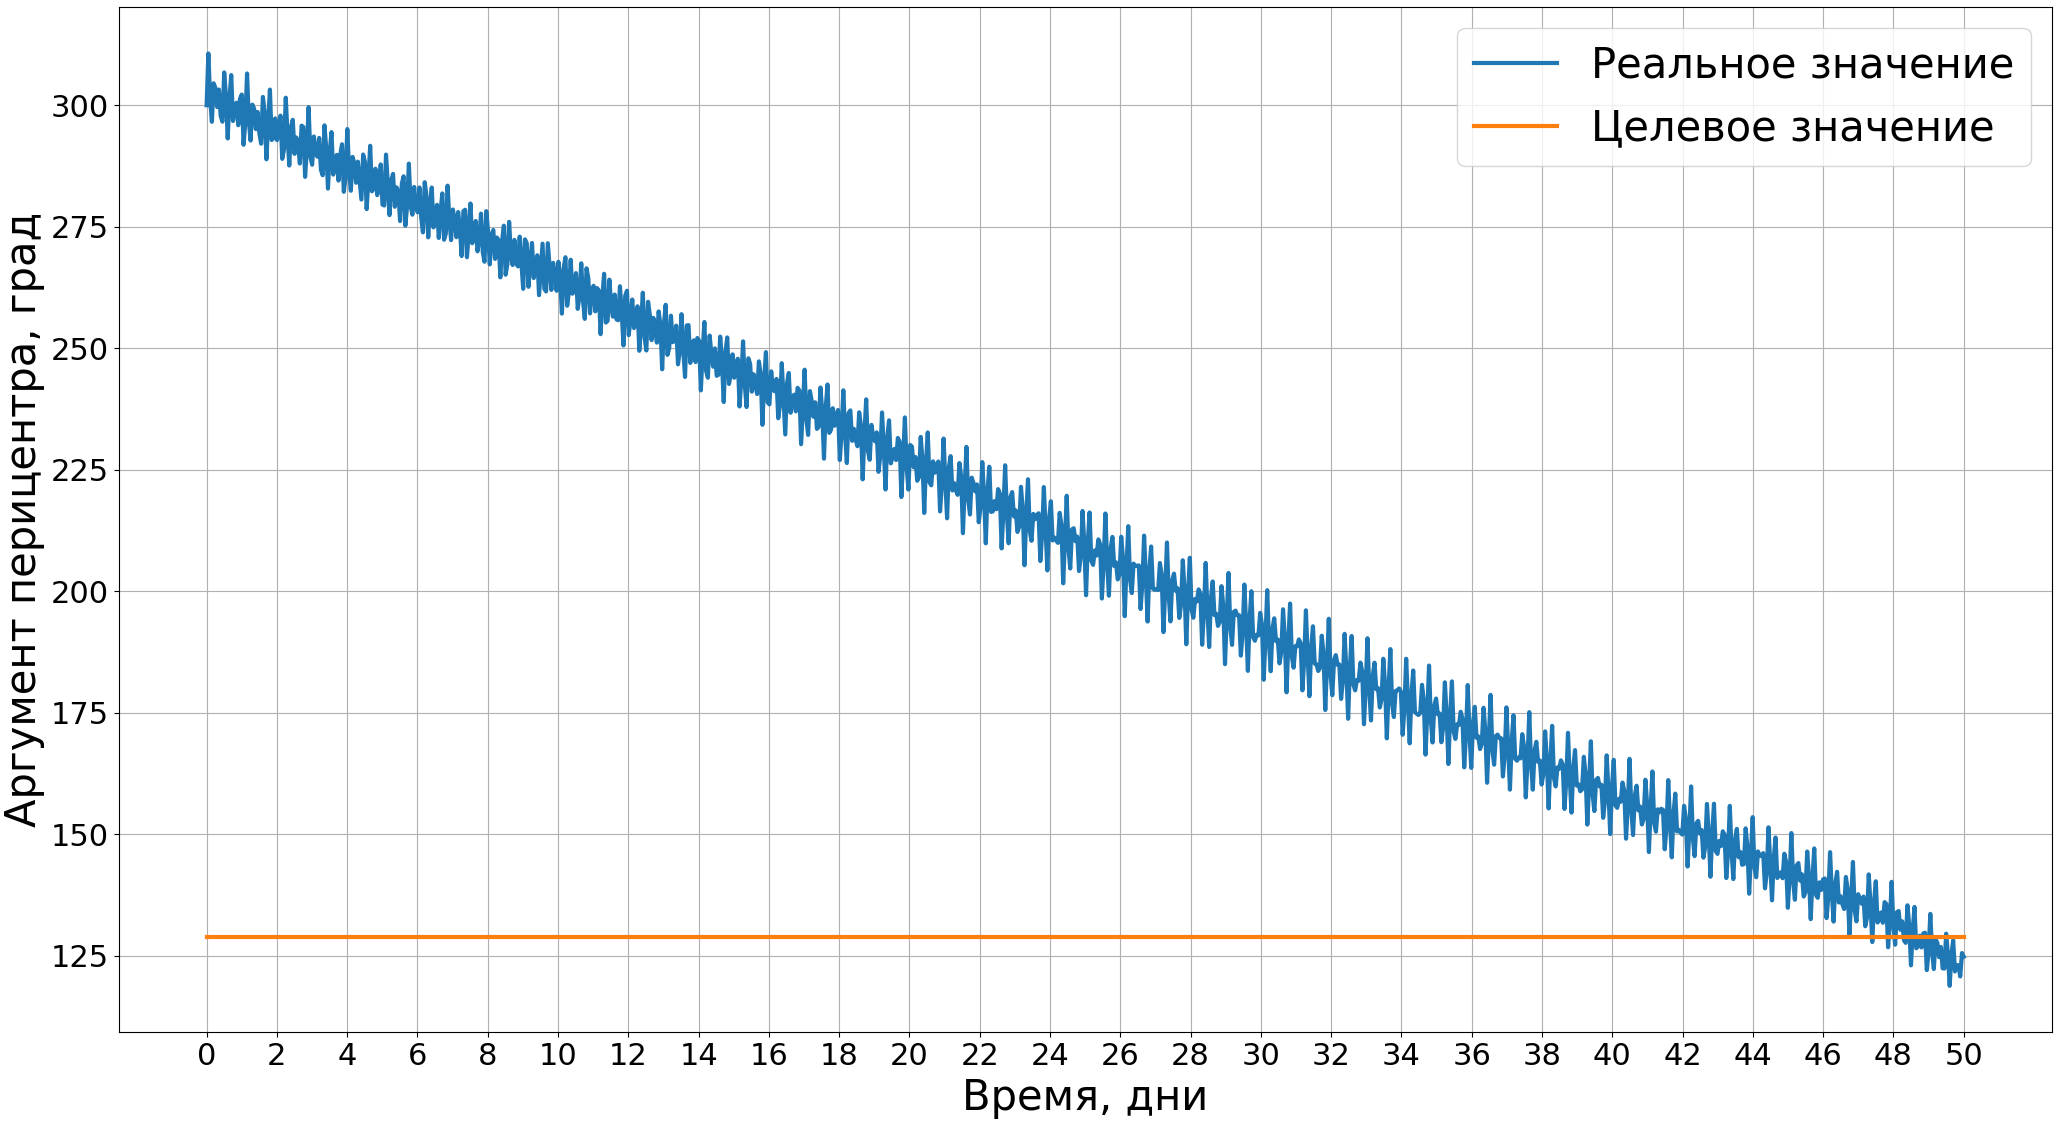
\includegraphics[height=0.37\textheight,keepaspectratio]{images/9/long_rend/w.png}
        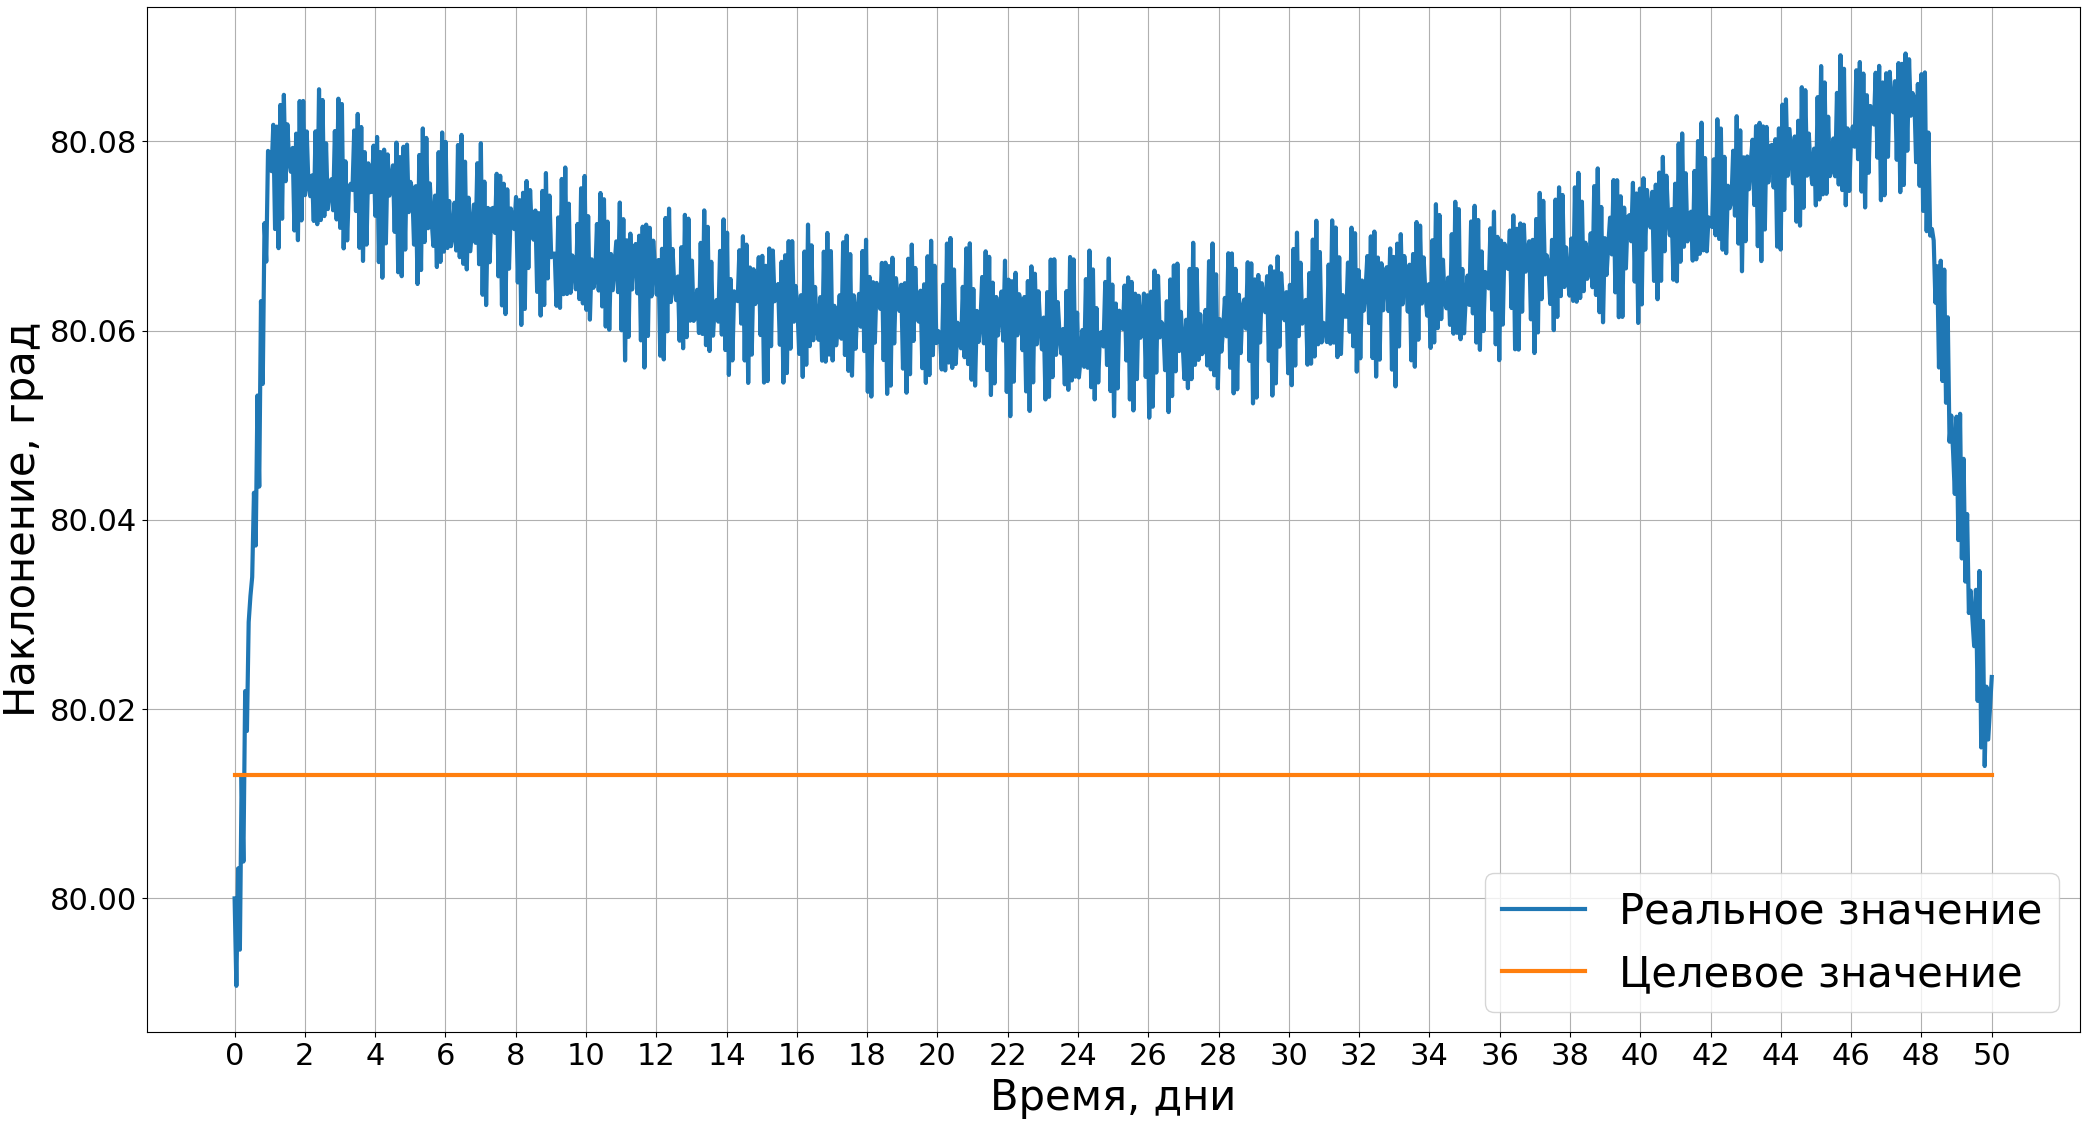
\includegraphics[height=0.37\textheight,keepaspectratio]{images/9/long_rend/i.png}
    \end{center}
  \end{column}

  % Правая колонка
  \begin{column}{0.50\textwidth}
    \begin{center}
        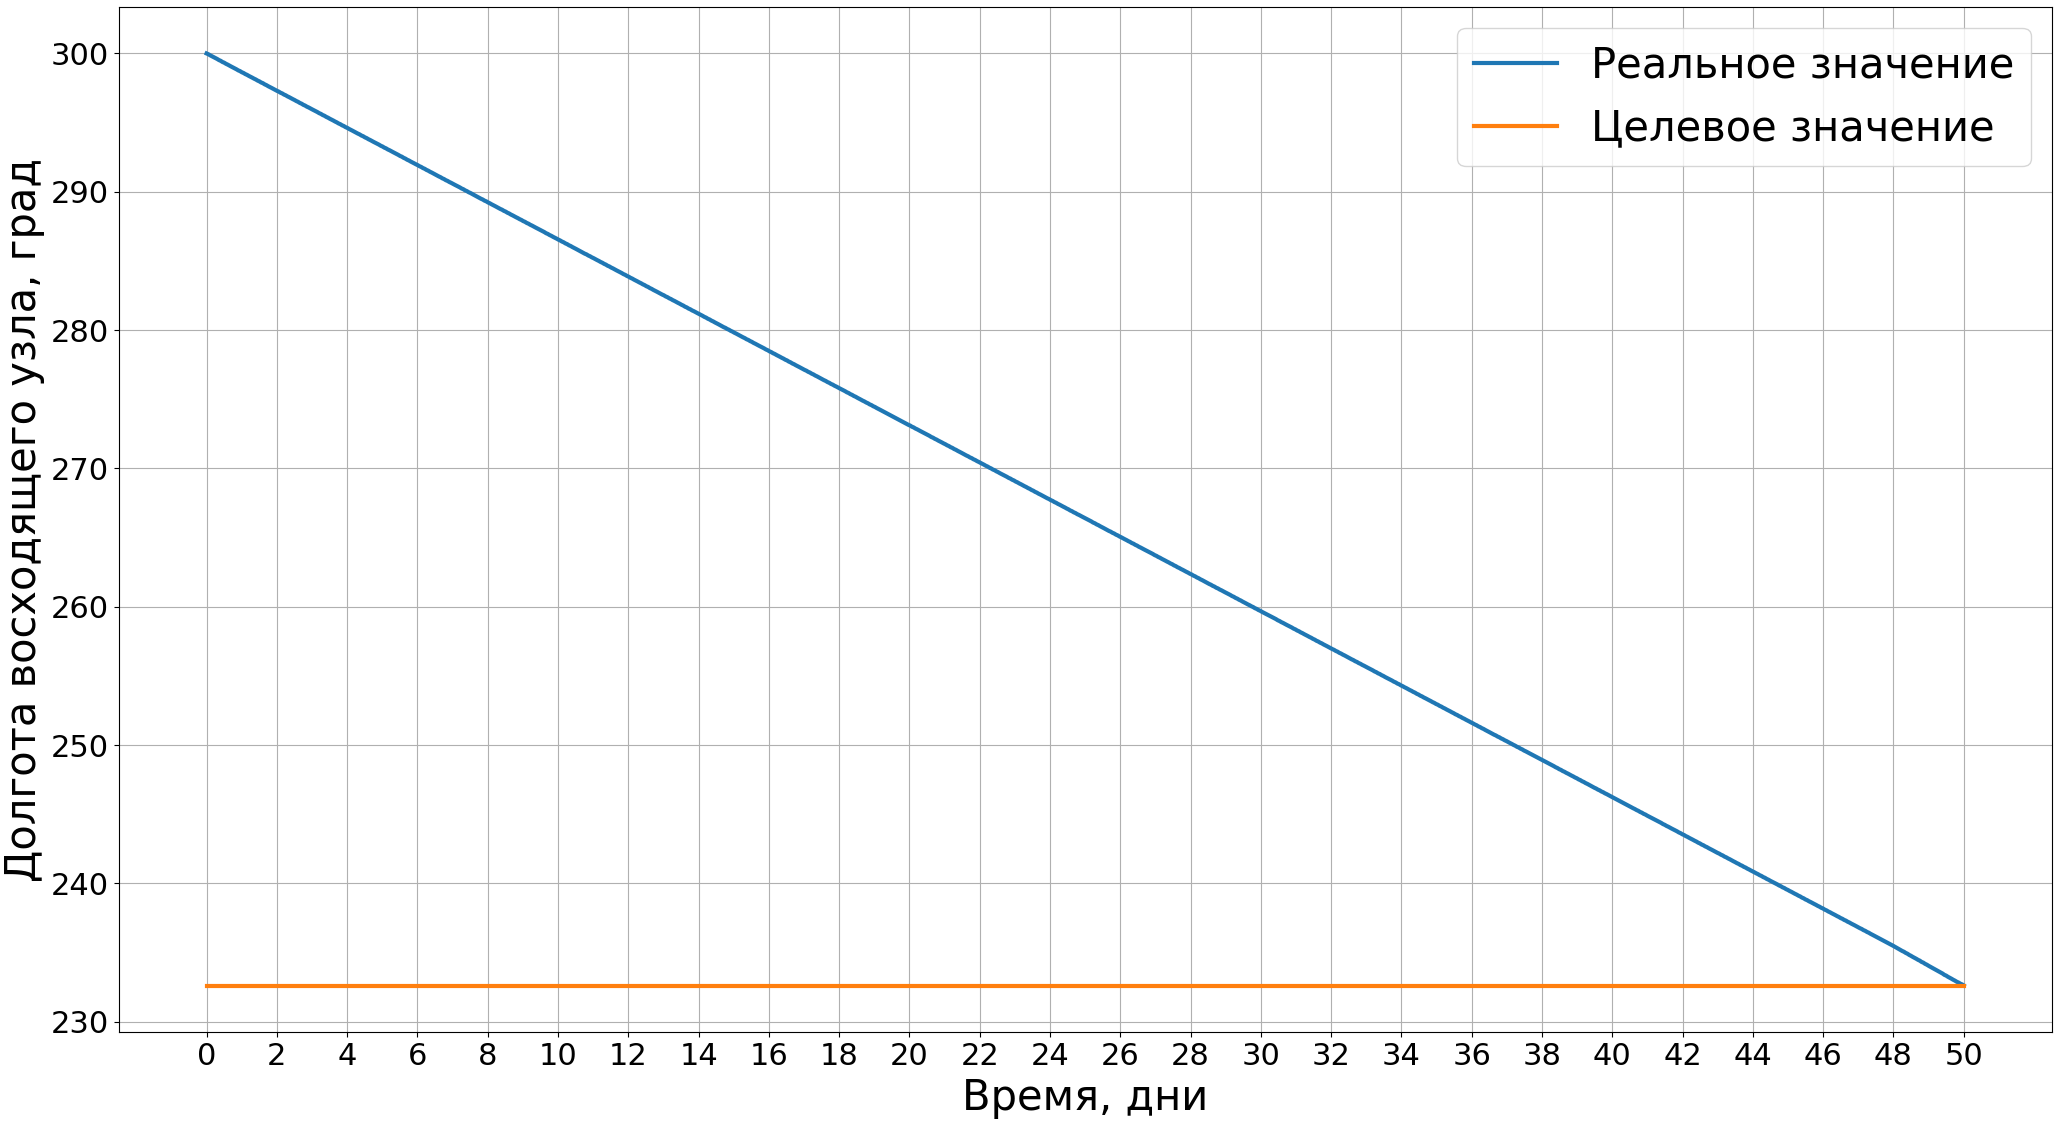
\includegraphics[height=0.37\textheight,keepaspectratio]{images/9/long_rend/raan.png}
        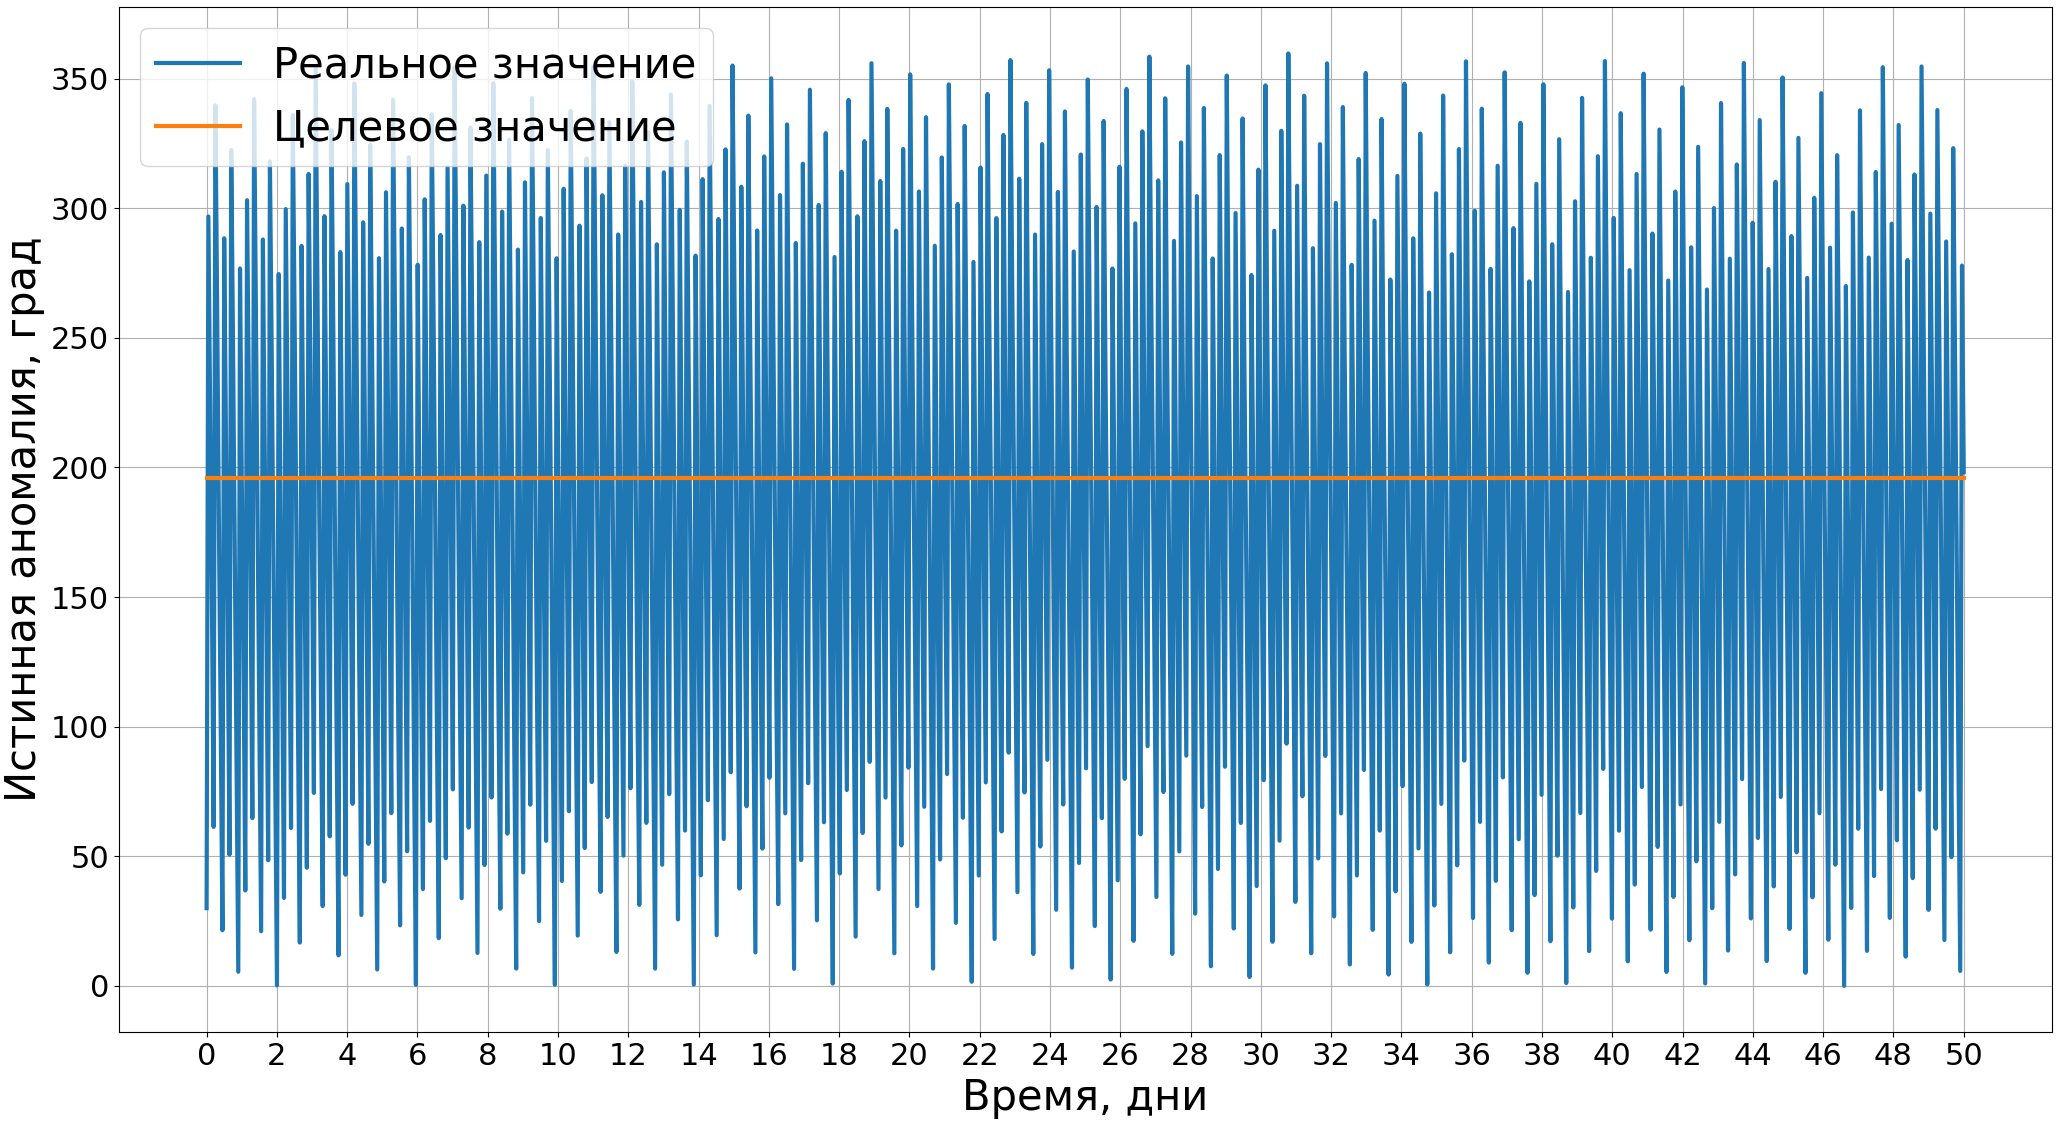
\includegraphics[height=0.37\textheight,keepaspectratio]{images/9/long_rend/nu.png}
    \end{center}
  \end{column}
\end{columns}
\end{frame}

\begin{frame}{Пример решения задачи встречи большой продолжительности}
\begin{center}
    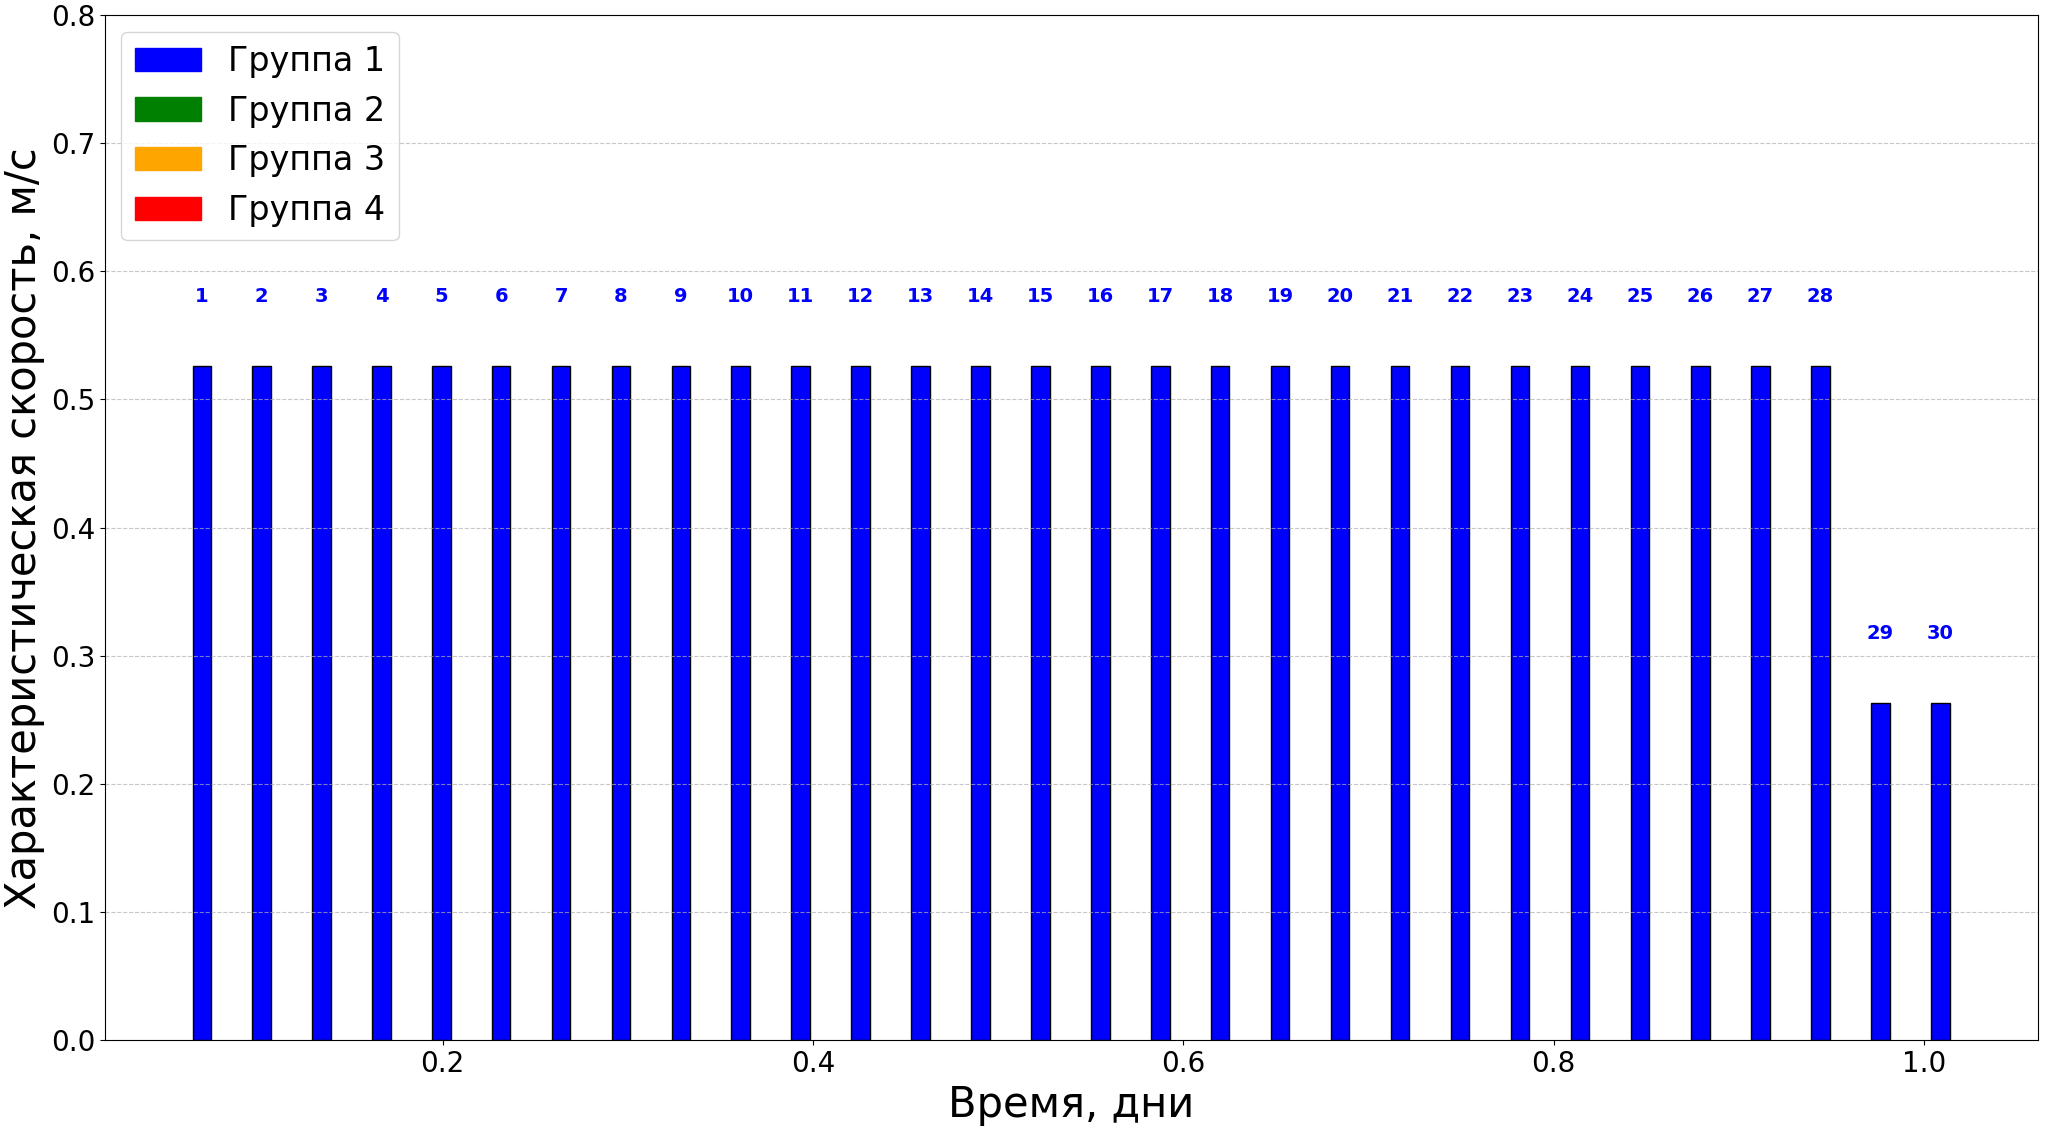
\includegraphics[height=0.4\textheight,keepaspectratio]{images/9/long_rend/v_distribution_1.png}
    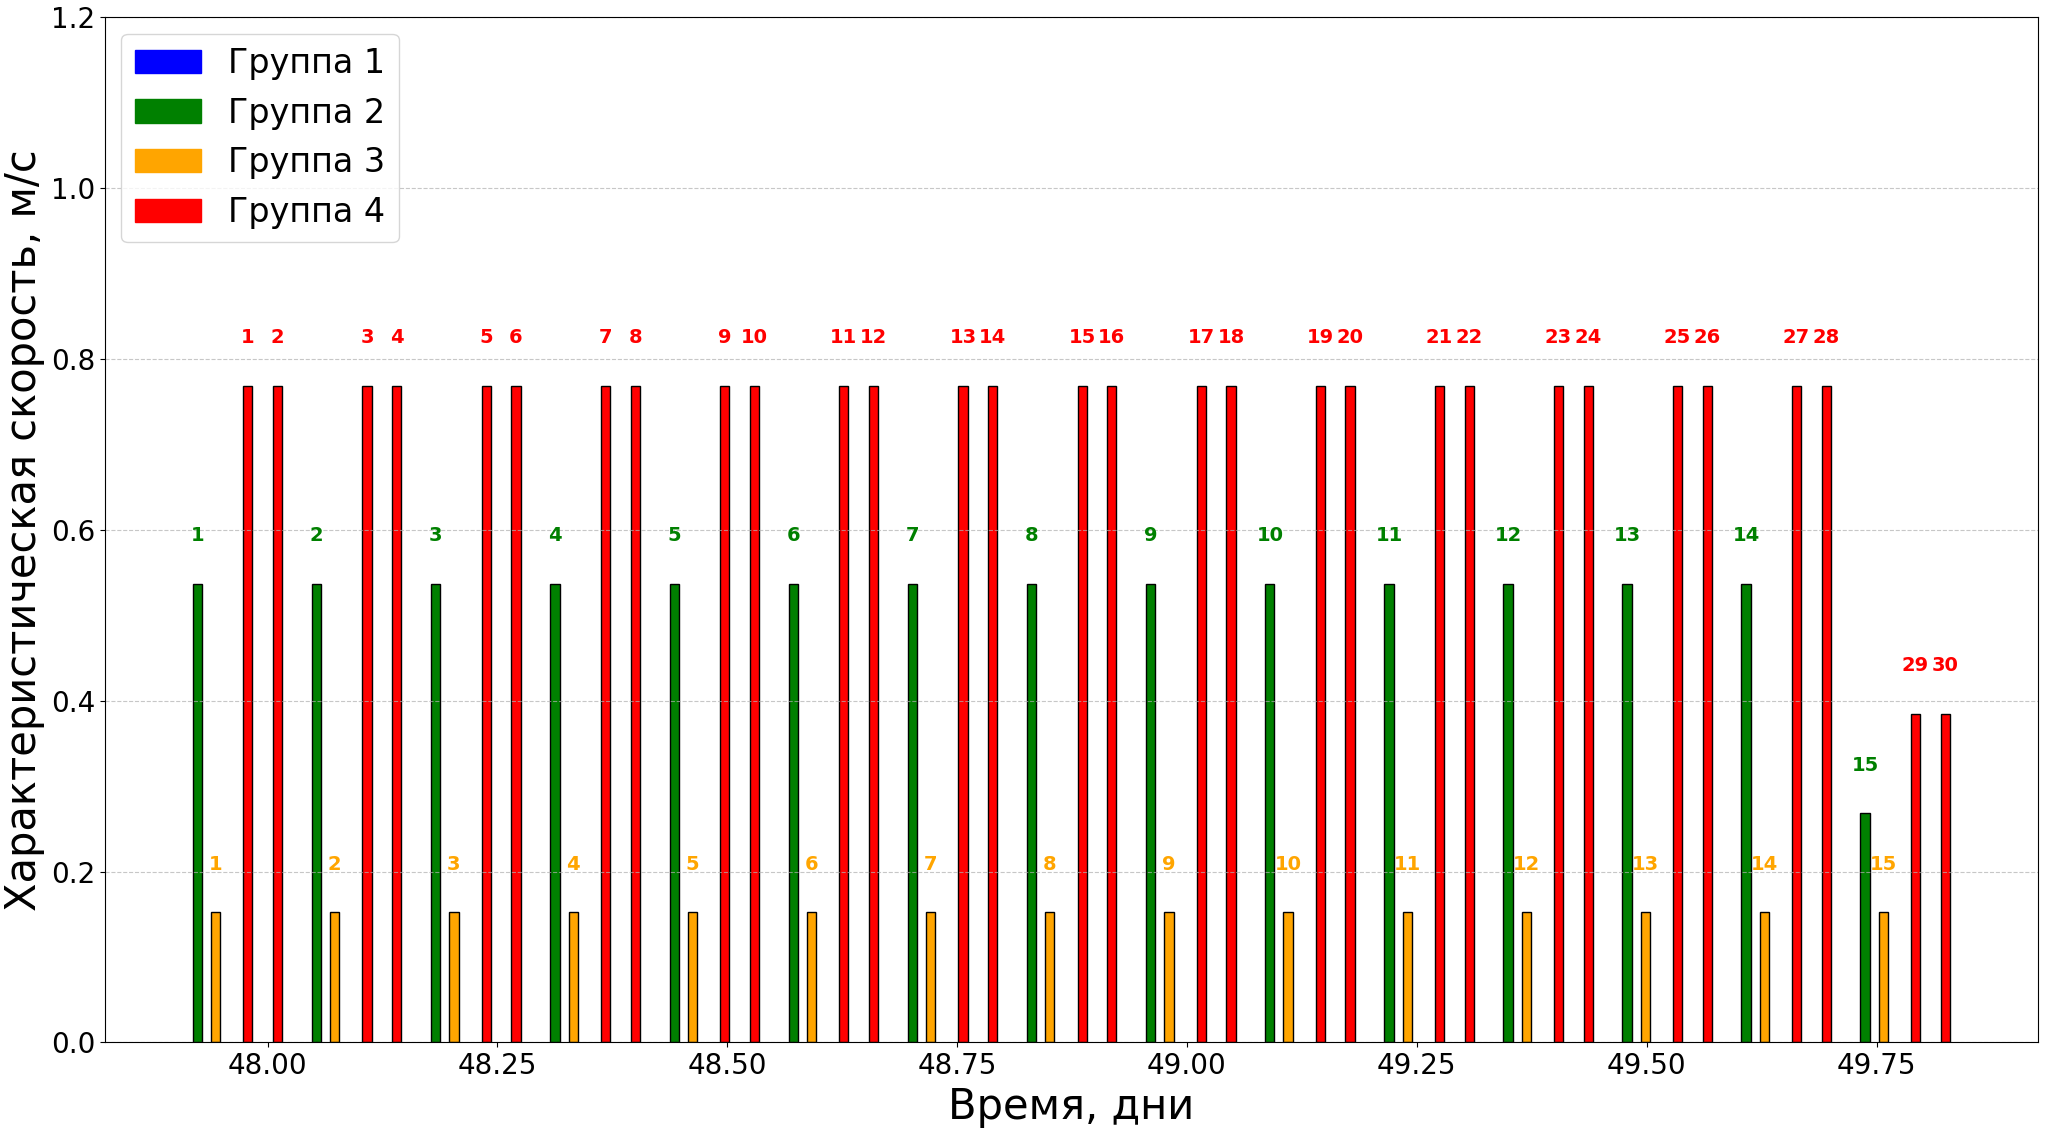
\includegraphics[height=0.4\textheight,keepaspectratio]{images/9/long_rend/v_distribution_2.png}
\end{center}
\end{frame}

\begin{frame}[allowframebreaks]{Источники}
  \begin{thebibliography}{9}

    \bibitem{DiPrinzio}
    DiPrinzio M. Methods of Orbital Maneuvering. – American Institute of Aeronautics and Astronautics, Inc., 2019.
    
  \end{thebibliography}
\end{frame}

\end{document}